\chapter{Evaluationen}
\label{ch:05_evaluation}

% Allgemeine Einleitung.
Nach der Definition der softwaretechnischen Realisierung und dem Aufzeigen erster Grenzen und Eigenheiten der
untersuchten Rendering-Paradigmen in Kapitel 4 werden die implementierten Architekturen isolierten Stresstests
unterzogen.
Das primäre Ziel dieses Kapitels liegt in der objektiven Quantifizierung der zuvor theoretisch beschriebenen
Performance-Engpässe unter systematischen Skalierung von Szenenkomplexität und Stil-Entropie.
Der erste Abschnitt definiert die methodischen Rahmenbedingungen sowie die technischen Spezifikationen des
Versuchsaufbaus, um eine belastbare Beantwortung der Forschungsfragen zu gewährleisten.
Darauf aufbauend erfolgt die schrittweise Datenauswertung anhand spezifischer Kontrollgruppen und der gezielten
Untersuchung vermuteter Performance-Engpässe, bevor ein abschließender Makro-Benchmark die gewonnenen Erkenntnisse
ganzheitlich evaluiert.


\section{Evaluationsmethodik \& Versuchsaufbau}
\label{sec:0501_evaluation_methodology}

% 5.1 Einleitung.
Das in Kapitel~\ref{ch:04_konzeption_realisierung} konzipierte Test-Framework fungiert im Folgenden als Messwerkzeug für die empirische Analyse der darin
implementierten Rendering-Pipelines.
Für die objektive und isolierte Betrachtung der verschiedenen postulierten Performance-Engpässe definiert der
vorliegende Abschnitt die methodischen Grundlagen.
Dies umfasst die Formulierung von Hypothesen, die exakte Spezifikation des Test-Systems und des
Variablen-Mappings sowie die Orchestrierung des Versuchsablaufs.

\subsection{{Zielsetzung und Hypothesen der Untersuchung}}
\label{subsec:050101_evaluation_tagets_and_hypothesis}

% Evaluationsziel
Wie in Kapitel~\ref{sec:0202_rendering_paradigms} dargelegt, weisen die theoretischen Architekturparadigmen des Forward-, Deferred-Uber- und
Deferred-Volume-Renderings spezifische Leistungsmerkmale auf.
Das primäre Ziel der nachfolgenden Testreihen besteht in der isolierten Quantifizierung dieser technologischen
Trade-offs.
Es sollen die individuellen Kipppunkte auf Hardware-Ebene lokalisiert und evaluiert werden.
Dadurch soll vermieden werden, eine Pipeline den anderen gegenüber als inhärent überlegen zu präsentieren.

% Technische Hypothesen.
Auf Basis der in Kapitel~\ref{ch:02_grundlagen} dargelegten theoretischen Faktenlage werden für die implementierten Rendering-Pipelines
spezifische Leistungshypothesen formuliert.
Diese Annahmen gilt es im Folgenden durch gezielte Evaluationen objektiv zu verifizieren oder zu falsifizieren.
Die empirische Untersuchung beleuchtet dabei gleichzeitig die hardwaretechnischen Grenzen und strukturellen Schwächen
des verwendeten Evaluations-Frameworks \ac{HyDra}.

% Hypothese Forward.
Für die als Referenz gewählte Single-Pass-Forward-Rendering-Pipeline werden zwei primäre Leistungsengpässe postuliert.
Auf \ac{GPU}-Ebene wird bei steigender Szenen- und Beleuchtungskomplexität erwartet, dass die Kombination aus
geometrischem Fragment-Overdraw und der multiplikativen algorithmischen Komplexität der direkten
Beleuchtungsberechnung von $\mathcal{O}(\text{Fragmente} \cdot \text{Lichter})$ (vgl.~\ref{eq:forward_shading_complexity}) zu signifikanten Leistungseinbußen führt
(\hypertarget{hyp:H1.1}{Hypothese H1.1}).
Hinsichtlich der \ac{CPU}-Auslastung wird angenommen, dass das \ac{CPU}-seitige Filtern und Zuordnen von Lichtquellen
pro Objekt sowie das hochfrequente Binden objektspezifischer Licht-Uniforms einen signifikanten \ac{API}-Overhead
provoziert, der die \ac{CPU}-Zuweisungszeit bei anwachsender Instanzenanzahl nicht-linear skalieren lässt
(\hypertarget{hyp:H1.2}{Hypothese H1.2})~\cite[Abschn.~1]{haradaForwardBringingDeferred2012}.

% Hypothese Deferred_Uber.
Für die Deferred-Pipeline mit einfachem Beleuchtungs-Pass (Single-Pass) und monolithischem Uber-Shader wird anhand
von Kapitel~\ref{subsec:020202_deferred_rendering} und~\ref{subsec:020303_warp_divergence_and_register_pressure} postuliert, dass
der signifikanteste Leistungsengpass bei einer hohen räumlichen Stil-Entropie auftritt
(\hypertarget{hyp:H2}{Hypothese H2}).
Wie in Kapitel~\ref{subsec:020303_warp_divergence_and_register_pressure} theoretisch hergeleitet, erzwingen feingranular gestreute \ac{NPR}-Effekte divergente
Code-Zweige (Warp-Divergence \& Registerdruck).
Diese kombinierten Hardware-Flaschenhälse zwingen die Architektur zu einer sequenziellen Abarbeitung der Pixel und
lassen eine messbare Degradation der Shading-Performance bei stark vermischten Effekten erwarten.

% Hypothese Deferred_Volumes.
Für die Deferred-Pipeline auf Basis von Light-Volumes (Deferred-Volume) postuliert \hypertarget{hyp:H3}{Hypothese H3},
anhand von Kapitel~\ref{subsec:020202_deferred_rendering} und~\ref{subsec:020302_memory_bandwidth}, dass diese
Architektur eine hohe Resilienz gegenüber räumlicher Stil-Entropie aufweist und die Branching-Problematik des
Uber-Shaders umgeht.
Der primäre Leistungsengpass dieser Methode wird stattdessen in der Sättigung der Speicherbandbreite vermutet
(vgl.\ Kap.~\ref{subsec:020302_memory_bandwidth}).

% Abgrenzung sonstiger Limits.
Im vorliegenden Kapitel werden die untersuchten Limitierungen ausschließlich auf Hardware-Leistungs-Ebene betrachtet.
Spezifische harte Implementierungsgrenzen der Pipelines (wie etwa die Uniform-Buffer-Limitierungen der Forward- und
Deferred-Uber-Architekturen) sowie etwaige künstlerische Qualitätsengpässe fließen nicht in die Messreihen ein.
Diese Aspekte wurden bereits in Kapitel~\ref{sec:0402_pipelines_and_restrictions} verortet und evaluiert.
Da weiterhin im Rahmen dieser Makro-Evaluation keine herstellerspezifischen Hardware-Profiler wie \textit{NVIDIA Nsight}
eingesetzt werden, um Mikrometriken wie exakte Cache-Hit-Raten oder Thread-Maskierungen auf Siliziumebene auszulesen,
werden die architektonischen Engpässe deduktiv aus den gemessenen Rendering-Laufzeiten abgeleitet.
Die benannten Ursachen sind daher stark korrelierende, theoretische Erklärungsmodelle für das beobachtete
Performance-Verhalten.

\subsection{{Systemkonfiguration und Variablen-Mapping}}
\label{subsec:050102_evaluation_configuration_and_variable_mapping}

% Einleitung
Im Folgenden werden die Referenzdaten der Testumgebung und des verwendeten Software-Stacks beschrieben.
Es werden die für die Testreihen angewendeten unabhängigen Variablen, abhängigen Variablen (Metriken) sowie die
entsprechenden Kontrollvariablen dargelegt und definiert.
Die referenzierten detaillierten tabellen sind hierzu sind im Anhang
unter~\ref{ch:AA_configuration_and_variable_mapping} zu finden.

% Einleitung zur Systemkonfiguration.
Die in Tabelle~\ref{tab:hardware_specs} aufgezeigten Hardware-Spezifikationen bestimmen die absoluten physikalischen
Leistungsgrenzen des Systems auf dem dies vorliegenden Versuche durchgeführt wurden.
Die in Tabelle~\ref{tab:software_specs} dokumentierten Software-Schnittstellen und Treiber-Versionen kontextualisieren
die \ac{CPU}-seitige Code-Basis sowie den grundlegenden \ac{API}-Overhead.

% Einleitung unabhängige Variablen.
Nach der Definition der Hardware- und Software-Spezifikationen erfordert das Evaluation-Design eine exakte Abgrenzung
der unabhängigen Variablen.
Diese Parameter manipuliert das Framework während der Testreihen systematisch.
Es sollen Leistungsgrenzen der Hardware isoliert provoziert werden.
Tabelle~\ref{tab:independent_vars} fasst das entsprechende Variablen-Mapping zusammen.

% Einleitung abhängigen Variablen.
Im direkten Gegenzug zu den manipulierten Parametern erfasst das Telemetrie-Modul des Frameworks eine Reihe
quantitativer Messgrößen.
Diese abhängigen Variablen bilden die empirische Datengrundlage der Evaluationen.
Die Aggregation der Daten pro Frame sowie deren tabellarische Aufarbeitung dienen der isolierten Beurteilung der
Hardware- und Softwareleistung für die spätere statistische Auswertung.
Tabelle~\ref{tab:dependent_vars} beschreibt die extrahierten Leistungs- und Szenenmetriken.
Die \ac{GPU}-Laufzeiten werden dabei über asynchrone Hardware-Queries ermittelt, um ein Blockieren der \ac{CPU}-Pipeline
zu verhindern.

% Einleitung Kontrollvariablen.
Den Abschluss des Variablen-Mappings bilden die Kontrollvariablen.
Diese Parameter definieren die statische Baseline des Frameworks.
Diese Werte bleiben konstant, um reproduzierbare Bedingungen für alle Messreihen zu gewährleisten, es sei denn, die
jeweilige Test-Suite überschreibt sie explizit als unabhängige Variable.
Tabelle~\ref{tab:controlled_vars} fasst die Standardkonfiguration der Kontrollvariablen zusammen.

\subsection{{Versuchsablauf}}
\label{subsec:050103_evaluateion_procedure}

% Aufwärmphase.
Vor der aktiven Datenaufzeichnung durchläuft das System eine obligatorische Warm-up-Phase von zehn Sekunden.
Dieser Prozess dient dazu, die Hardware-Caches und Textur-Caches
aufzubauen~\cites[Kap.~18.4, Abschn.~\textit{Memory Issues}]{akenine-mollerRealtimeRendering2019}
[]{NVIDIATuringArchitectureWhitepaper}.
Hierdurch werden inkonsistente Frametimes, die durch asynchrone Ladevorgänge, späte Speicherallokationen oder
aufgeschobene Statusänderungen des Grafiktreibers in den ersten Frames
entstehen~\cite[Kap.~18.4.2, Abschn.~\textit{State Changes}]{akenine-mollerRealtimeRendering2019},
für die Messung exkludiert.
Während der Wechsel zwischen Rendering-Pipelines oder beim Voranschreiten abhängiger Schritt-Variablen wird ebenfalls eine
Warm-up-Pause von zehn Sekunden erzwungen.


% Sampling.
Nach der Warm-up-Phase startet die Sampling-Phase mit einer festgelegten Dauer von \texttt{1000} Frames.
Die Kamera wird eingefroren (Ausnahme: Evaluation 5.6).
Das Telemetrie-Modul fragt nun jede der definierten abhängigen Variablen pro Frame ab und akkumuliert die Rohdaten in
dedizierten Arrays zur späteren Exportierung.

% Datenaufbereitung.
Die final präsentierten Graphen und Messergebnisse basieren auf arithmetischen Mittelwerten der Sampling-Phase.
Identifikation und Bereinigung unvorhersehbarer Micro-Stutterer (\textit{Frame-Rate Spikes}) erfolgt durch die
Standardabweichung der Frame-Zeiten~\cite[Abschn.~8.5.2.2]{gregoryGameEngineArchitecture2018}.
Für jede Parameter-Konfiguration bildet die Menge der erfassten Frame-Metriken den initialen Datensatz $X$.
Aus diesem werden gruppenbasiert der empirische Mittelwert $\mu$ sowie die Standardabweichung $\sigma$ berechnet.
Ein individueller Messwert $x_i \in X$ wird ausschließlich dann in die finale Kurvengenerierung einbezogen, sofern die
folgende Bedingung erfüllt ist:

\begin{equation}
    \mu - 3\sigma \le x_i \le \mu + 3\sigma
\end{equation}

Datenpunkte außerhalb dieses Intervalls klassifiziert der Algorithmus als statistische Ausreißer und verwirft diese für
die finale Auswertung.
Dieser Schritt garantiert, dass die später präsentierten Messdaten das rein architektonische und algorithmische
Skalierungsverhalten der Rendering-Pipelines abbilden.


\section{{Geometrische Dichte und Overdraw}}
\label{sec:0502_geometry_eval}

Im Rahmen des nachfolgenden Kapitels werden Benchmarks und Erkenntnisse präsentiert, die dazu dienen, geometriebedingte
Performance-Bottlenecks innerhalb der untersuchten Rendering-Pipelines zu evaluieren.
Der Fokus liegt primär auf der Isolation der \textit{Hardware-Rasterize} und der \ac{CPU}-Draw-Call-Aufwände.

\subsection{{Level of Detail (Mikro-Geometrie)}}
\label{subsec:050201_lod_eval}

% Einleitung.
Das Ziel dieser Testreihe besteht in der Isolation des Hardware-Rasterizers zur Evaluierung der geometrischen Basis-Last.
Konkret soll das absolute Limit der Vertex-Verarbeitung (\textit{Triangle Throughput}) identifiziert und der Einfluss des
\ac{G-Buffer}-Speicherdurchsatzes isoliert bewertet werden.
Zu diesem Zweck wird die Pipeline einem reinen Geometrie-Stresstest ohne Beleuchtungseinflüsse ($N_{\text{Light}} = 0$)
ausgesetzt, um zu prüfen, ob die massiven Speicherschreibvorgänge der Deferred-Pipelines bei hoher Dreiecks-Dichte im
Vergleich zur Forward-Pipeline einen signifikanten Bandbreiten-Engpass
erzeugen \cite[S.~55]{burnsVisibilityBufferCacheFriendly2013}.

% Versuchs-Setup
\begin{center}
    \small
    \colorbox{gray!5}{\parbox{0.95\textwidth}{
        \centering
        \vspace{2mm}
        {\sffamily\bfseries Versuchs-Setup} \\[1.5ex]
        \begin{tabularx}{0.9\textwidth}{>{\sffamily}l X}
            Unabhängige Variable:    & Geometrischer Detailgrad ($LOD \in \{0, \dots, 4\}$) \\
            Skalierung (Dreiecke):   & $24.000$ bis $16{,}38\text{ Mio.}$ Dreiecke \\
            Kontrollvariablen:       & $N_{\text{Inst}} = 2.000$, $N_{\text{Light}} = 0$, $C_{\text{Floor}} =
            \text{Deaktiviert}$, $\text{Culling} = 0\%$, Statische Kamera \\
            Zielgrößen:              & \ac{GPU}-Gesamtlaufzeit ($t_{\text{GPU}}$), Dispatch-Laufzeit ($t_{\text{CPU}}$)
        \end{tabularx}
        \vspace{2mm}
    }}
\end{center}

% Deskriptive Beobachtung
Wie aus den Ergebnissen in Abbildung~\ref{fig:5_2_1_bottleneck_divergence} zu erkennen ist, verhalten sich die
verschiedenen Rendering-Pipelines nahezu identisch und skalieren auch bei erhöhtem Detailgrad ($\text{\ac{LOD}}$)
äquivalent, sowohl in Bezug auf die \ac{GPU}- als auch die \ac{CPU}-Auslastung.
Weiterhin ist zu beobachten, dass sich die \ac{GPU}-Gesamtlaufzeit ($t_{\text{GPU}}$) nahezu linear zur absoluten
Dreiecksanzahl ($\mathcal{O}(N)$) verhält, wohingegen die Dispatch-Laufzeit der \ac{CPU}
weitestgehend konstant ($\mathcal{O}(1)$) bleibt.

% Ergebnis Graph
\begin{figure}[htbp]
    \centering
    
\includegraphics[width=0.7\linewidth]{abbildungen/5-2-1_bottleneck_divergence}
    \caption[Messung der GPU- und CPU-Laufzeiten bei LOD-Skalierung]{Messung der GPU- und CPU-Laufzeiten bei einer
        $\text{LOD}$-Skalierung von 24.000 bis 16,38 Mio. Dreiecken und einer konstanten Objektanzahl von 2.000.}
    \label{fig:5_2_1_bottleneck_divergence}
\end{figure}

% Deduktion.
Die ermittelte Laufzeit-Parität zwischen den Pipelines widerlegt die Hypothese der hohen Speicher- und
Bandbreitenkosten für reine Geometrieszenarien~\cite[S.~905]{akenine-mollerRealtimeRendering2019}.
Das Füllen der breiteren Deferred-Buffer erzeugt gegenüber dem Forward-Buffer keinen limitierenden Bandbreiten-Overhead
auf dem \ac{VRAM}-Bus.

% Limitation.
Es sei jedoch methodisch angemerkt, dass eine rein geometrische Skalierung auf konstantem Raum nur bedingt
geeignet ist, um die \ac{VRAM}-Speicherbandbreite zu sättigen.
Die extrem hohe Dreiecksdichte bei $LOD = 4$ ($16{,}38\text{ Mio.}$ Dreiecke auf $2.000$ Instanzen bei 1080p) führt
dazu, dass die Größe der verarbeiteten Dreiecke den Subpixel-Bereich erreicht oder sogar
unterschreitet~\cite[S.~1]{fatahalianReducingShadingGPUs2010}.
Die Hardware stößt bei der Transformation dieser winzigen Dreiecke an ihre Kapazitätsgrenze, noch bevor
eine signifikante Anzahl von Fragmenten erzeugt werden kann, die den \ac{VRAM}-Bus überhaupt belasten
würden~\cites[Kap.~18.2.3]{akenine-mollerRealtimeRendering2019}[Folie~\textit{Tiny triangles}]{Karis_Nanite_SIGGRAPH_Advances_2021_final}.

\subsection{{Objektanzahl}}
\label{subsec:050202_obejct_count_eval}

% Einleitung.
Das Ziel der folgenden Testreihe besteht in der Isolation der \ac{CPU}-Architektur.
In der vorliegenden Untersuchung werden die Draw-Call-Generierung sowie die Ausführungszeit des logischen Szenen-Passes
(Frustum Culling, Sichtbarkeitsprüfung und Matrix-Updates) durch eine schrittweise Skalierung der Geometrie-Instanzen
evaluiert.
Die Durchführung des Tests erfolgt ohne Beleuchtungseinflüsse ($N_{\text{Light}} = 0$) und bei minimalem geometrischen
Detailgrad ($LOD = 0$, 12-Dreieck-Würfel), um potenzielle \ac{GPU}-Engpässe zu eliminieren und eine isolierte
Betrachtung der Host-Seite (\ac{CPU}) zu gewährleisten.
Es wird primär die Hypothese geprüft, ob der \ac{CPU}-Overhead das Gesamtsystem limitiert, bevor die \ac{GPU}
vollständig ausgelastet ist, und inwiefern architektonische Unterschiede zwischen den Rendering-Pipelines im
Dispatch-Prozess auf der Host-Seite (\ac{CPU}) existieren.

% Aufbau.
\begin{center}
    \small
    \colorbox{gray!5}{\parbox{0.95\textwidth}{
        \centering
        \vspace{2mm}
        {\sffamily\bfseries Versuchs-Setup} \\[1.5ex]
        \begin{tabularx}{0.9\textwidth}{>{\sffamily}l X}
            Unabhängige Variable:    & Instanzen-Anzahl ($N_{\text{Inst}} \in \{1.000, \dots, 50.000\}$) \\
            Dynamische Variable:     & Kamera-Distanz (Skaliert proportional zu $N_{\text{Inst}}$ zur Vermeidung von
            Culling-Verzerrungen) \\
            Kontrollvariablen:       & $LOD = 0$, $N_{\text{Light}} = 0$, $C_{\text{Floor}} =
            \text{Deaktiviert}$ \\
            Zielgrößen:              & Logik-Laufzeit ($t_{\text{Logic}}$), Dispatch-Laufzeit ($t_{\text{Dispatch}}$)
        \end{tabularx}
        \vspace{2mm}
    }}
\end{center}

% Beobachtung.
Die Ergebnisse in Abbildung~\ref{fig:5_2_2_cpu_scaling_logic_vs_render} zeigen, dass sowohl die Laufzeiten des logischen
Szenen-Passes ($t_{\text{Logic}}$) als auch die Dispatch-Laufzeiten ($t_{\text{Dispatch}}$) mit der Instanzenanzahl
korrelieren, wobei die jeweiligen Steigungsraten signifikant divergieren.
Der Anstieg von $t_{\text{Dispatch}}$ verläuft zwar linear, verbleibt jedoch selbst bei einer Volllast von $50.000$
Instanzen mit ca. \qty{7,8}{\milli\second} über alle Rendering-Pipelines hinweg stabil und effizient.
Im Gegensatz dazu weist $t_{\text{Logic}}$ ein deutlich steileres Anstiegsverhalten auf, wobei sich die Forward-Pipeline
bei steigender Last zunehmend von den Deferred-Pipelines entkoppelt: In der Traversierung des logischen Szenen-Passes
(State-Changes/Culling) generiert die Forward-Architektur eine messbar höhere \ac{CPU}-Last als die
Deferred-Äquivalente.

% Ergebnis Graph.
\begin{figure}[htbp]
    \centering
    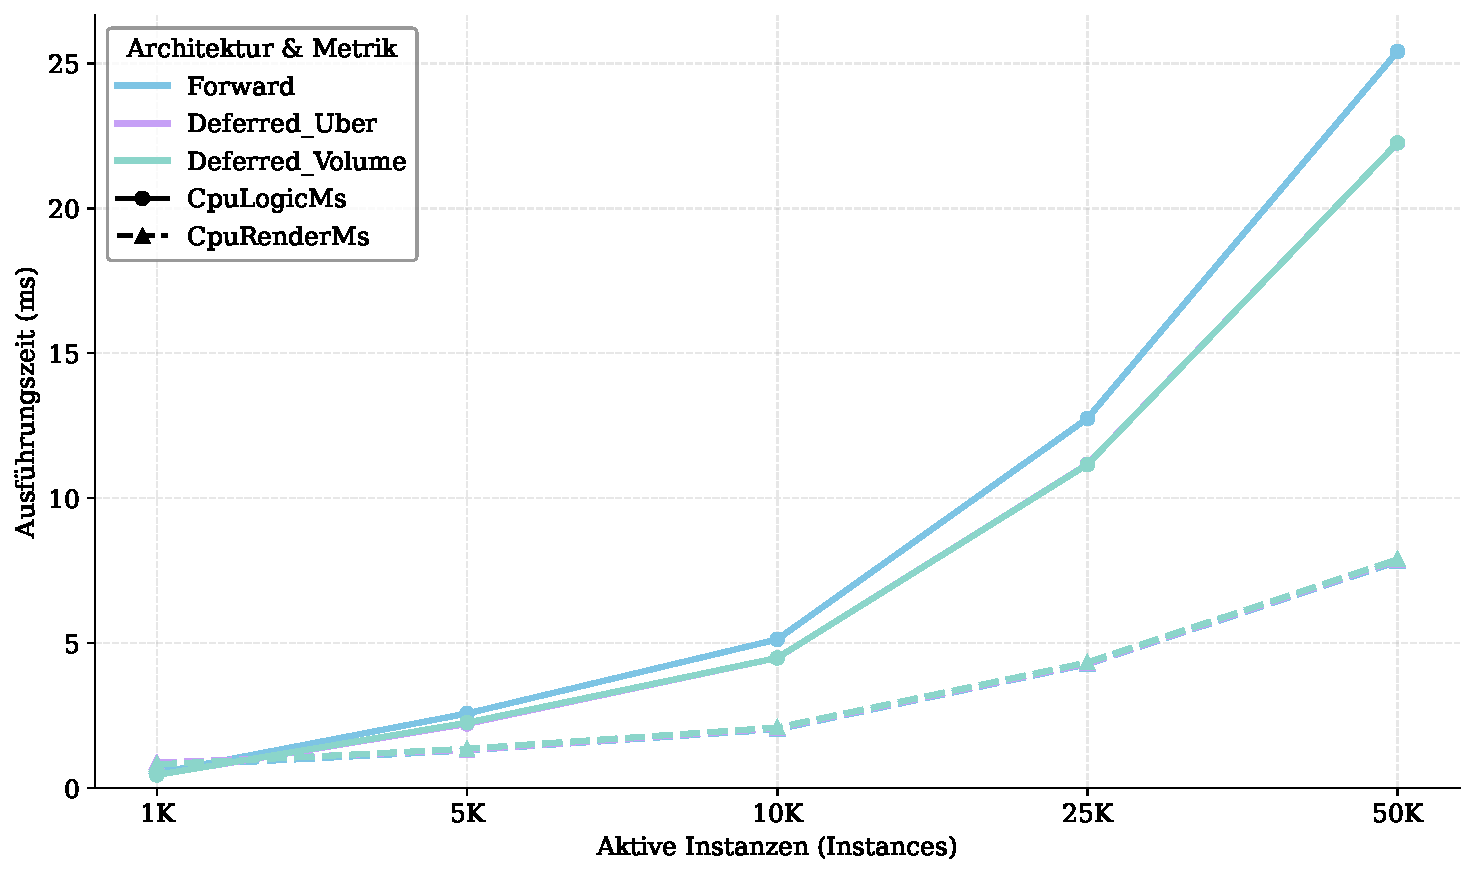
\includegraphics[width=0.85\linewidth]{abbildungen/5_2_2_cpu_scaling_logic_vs_render}
    \caption[Messung von Logik- und Dispatch-Laufzeiten bei Instanzenskalierung]{Messung von Logik-Laufzeit ($t_{\text{Logic}}$) und
    Dispatch-Laufzeit ($t_{\text{Dispatch}}$) bei
    einer Skalierung von 1.000 bis 50.000 Instanzen.}
    \label{fig:5_2_2_cpu_scaling_logic_vs_render}
\end{figure}

% Deduktion.
Die Analyse ergibt, dass die reine \ac{API}-Befehlsübermittlung an die Grafikkarte bei keinem der untersuchten
Rendering-Paradigmen einen primären Engpass darstellt.
Darüber hinaus kann beobachtet werden, dass die umfangreichen mathematischen Operationen (Frustum Culling,
\ac{MVP}-Matrix-Updates) die Datenverarbeitung auf der \ac{CPU} hier weitaus größer belasten.
Das Forward Rendering weist in diesem Kontext eine geringere Skalierbarkeit auf, da es pro Objekt auf der \ac{CPU} eine
Lichtliste evaluieren und binden muss~\cite[S.~891]{akenine-mollerRealtimeRendering2019}.
Wie~\textcite[S.~1]{Thaler2011DeferredRendering} beschreibt, müssen bei Single-Pass-Forward-Architekturen für jedes
Objekt zunächst alle beeinflussenden Lichtquellen gesucht werden.
Dieser Suchlauf kostet kontinuierlich \ac{CPU}-Zeit, auch wenn er bei $N_{\text{Light}} = 0$ für alle $N_{\text{Inst}}
= 50.000$ Objekte vollständig ins Leere läuft.
Das schlechtere Skalierungsverhalten der Forward-Pipeline bei verarbeitung des logischen Szenen-Passes afu der \ac{CPU}
verifiziert somit \hyperlink{hyp:H1.2}{Hypothese H1.2}.

% Limitationen.
Dies stellt gleichzeitig eine architektonische Limitation des genutzten Frameworks dar, da eine alternative
Implementierung des Forward Renderings in mehreren Pässen (ein Render-Pass pro Lichtquelle) diese spezifische
Suchlogik umgangen hätte (Multi-Pass-Forward)~\cite[S.~1]{Thaler2011DeferredRendering}.

\subsection{{Overdraw-Dichte}}
\label{subsec:050203_overdraw_eval}

% Einleitung.
Der folgende Versuch zielt darauf ab, den Einfluss extremer geometrischer Tiefenkomplexität (Overdraw) auf die
Speicherbandbreite der \ac{GPU} zu evaluieren.
Zu diesem Zweck wird $N_{\text{Inst}}$ auf engstem Raum ($r_{\text{Spawn}} = 30{,}0$) signifikant erhöht, um eine
substanzielle Z-Achsen-Stapelung zu erzwingen.
Aufgrund der Tatsache, dass Deferred Rendering beim Beschreiben des \ac{G-Buffer}s signifikant mehr
\ac{VRAM}-Bandbreite benötigt als Forward Rendering, wird eine Prüfung durchgeführt, ob ein hoher Overdraw-Faktor
($O_{\text{Draw}}$) die Deferred-Pipelines im Vergleich unverhältnismäßig stark ausbremst (Bandbreiten-Sättigung durch
massives Überschreiben von Pixeln).

% Aufbau.
\begin{center}
    \small
    \colorbox{gray!5}{\parbox{0.95\textwidth}{
        \centering
        \vspace{2mm}
        {\sffamily\bfseries Versuchs-Setup} \\[1.5ex]
        \begin{tabularx}{0.9\textwidth}{>{\sffamily}l X}
            Unabhängige Variable:    & Instanzen-Anzahl ($N_{\text{Inst}} \in \{2.000, \dots, 32.000\}$) \\
            Metrik (X-Achse):    & Theoretischer Overdraw-Faktor (($\approx 1{,}1$ bis $18{,}1$)) \\
            Kontrollvariablen:       & Fixer Radius ($r_{\text{Spawn}} = 30{,}0$), $\ac{LOD} = 1$, $N_{\text{Light}} =
            0$ \\
            Zielgröße:               & \ac{GPU}-Gesamtlaufzeit ($t_{\text{GPU}}$)
        \end{tabularx}
        \vspace{2mm}
    }}
\end{center}

% Beschreibung.
Obwohl alle analysierten Rendering-Pipelines einen messbaren Anstieg der \ac{GPU}-Ausführungszeit aufweisen, sind, wie
in Abbildung~\ref{fig:5_2_3_overdraw_fillrate_scaling} zu beobachten, die Abweichungen untereinander minimal.
Des Weiteren ist festzustellen, dass alle Rendering-Pipelines nahezu linear skalieren.

% Ergebnis Graph
\begin{figure}[htbp]
    \centering
    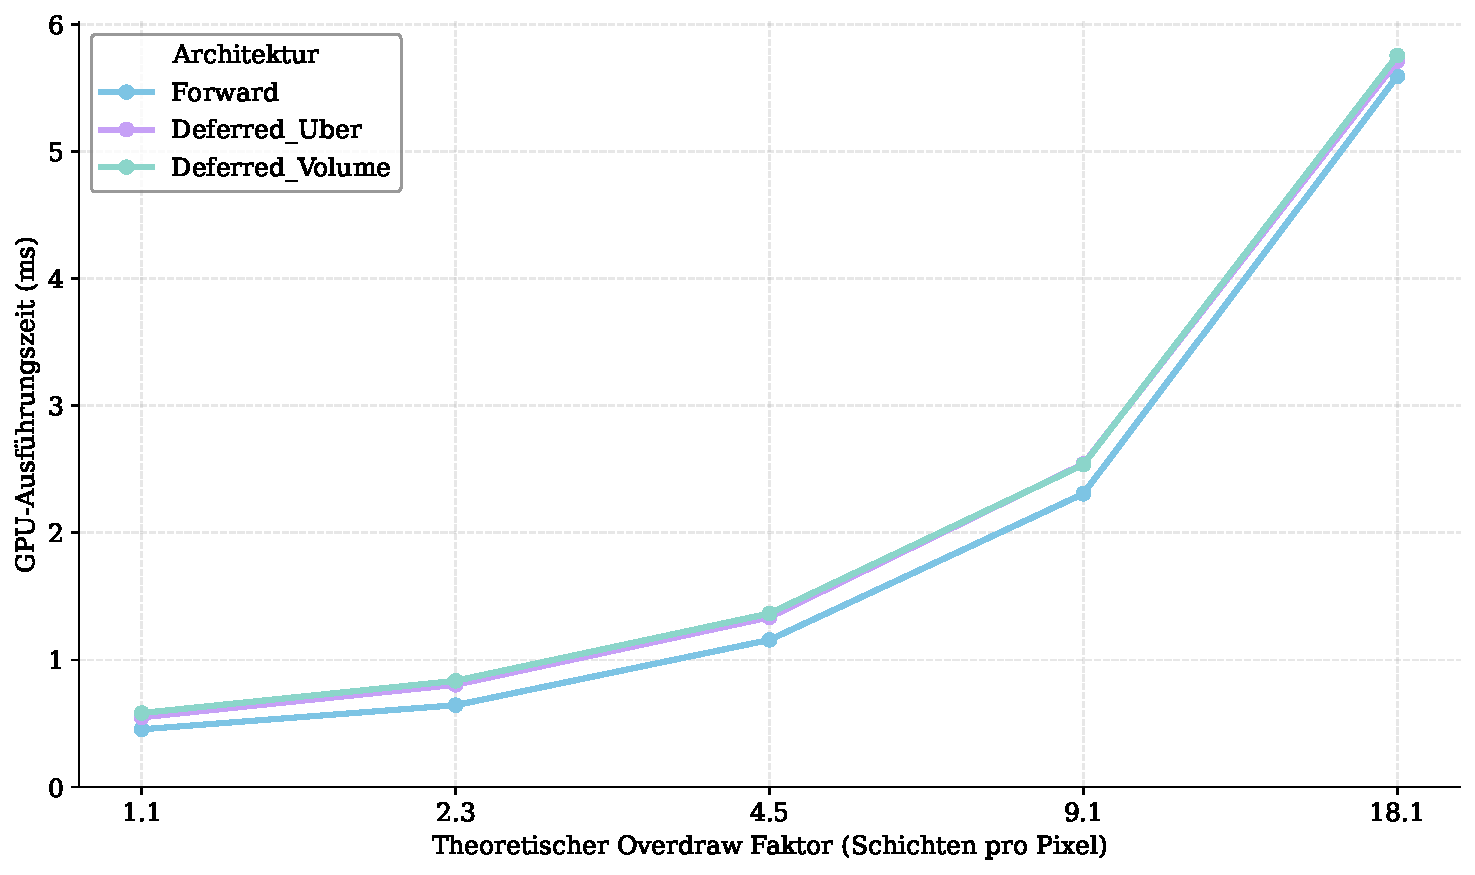
\includegraphics[width=0.85\linewidth]{abbildungen/5_2_3_overdraw_fillrate_scaling}
    \caption[Messung der GPU-Ausführungszeit bei Overdraw-Skalierung]{Messung der GPU-Ausführungszeit in Abhängigkeit vom
    theoretischen Overdraw-Faktor (1,1 bis 18,1 Schichten pro Pixel) bei einer Skalierung von 2.000 bis 32.000
    Instanzen.}
    \label{fig:5_2_3_overdraw_fillrate_scaling}
\end{figure}

% Deduktion
Die nahezu deckungsgleichen Kurven demonstrieren, dass die umfangreichen \ac{G-Buffer}-Schreibvorgänge selbst bei einem
äußerst hohen Overdraw keine \ac{VRAM}-Blockade induzieren.
Da opake Geometrie gerendert wird, testet die \ac{GPU}-Hardware die Tiefe bereits vor dem eigentlichen Fragment-Shader.
Es ist zu konstatieren, dass verdeckte Pixel-Fragmente mittels \textit{Early-Z} (vgl.\ Kapitel~\ref{subsec:020301_overdraw})
auf Siliziumebene verworfen werden, bevor kostspielige
Schreiboperationen in den Framebuffer oder \ac{G-Buffer} stattfinden. \cite[S. 801]{akenine-mollerRealtimeRendering2019}


\section{{Bandbreite und Auflösung}}
\label{sec:0503_brandwidth_resolution_eval}

In dem nachfolgenden Kapitel werden Benchmarks und Erkenntnisse präsentiert, die dazu dienen, die
bandbreitenspezifischen Limitierungen auszuloten.
Im Rahmen der Analyse werden die \ac{API} und die Speicherkosten des \ac{G-Buffer}s sowie der zunehmende \ac{ALU}-Aufwand des
Forward-Renderings betrachtet.

\subsection{{Auflösung}}
\label{subsec:050301_resolution_eval}

% Einleitung.
Der folgende Versuch zielt darauf ab, den Einfluss der Framebuffer-Auflösung (und der damit verbundenen Pixel-Anzahl)
auf die \ac{VRAM}-Füllrate und den Shading-Aufwand zu untersuchen.
Sowohl die Geometrie als auch die Lichtverhältnisse bleiben auf einen Standard von $N_{\text{Light}} = 200$ Lichtern und
$N_{\text{Inst}} = 5.000$ Objekt-Instanzen festgelegt.
Im Rahmen der Evaluierung werden ausschließlich die Auflösung und damit gerenderten Pixel analysiert.
Da Deferred Rendering die Beleuchtung strikt im 2D-Screen-Space berechnet, wird erwartet, dass die Kosten an die
Pixelanzahl gekoppelt sind~\cite[Abschn.~9.2]{Chapter9Deferred}.

% Aufbau.
\begin{center}
    \small
    \colorbox{gray!5}{\parbox{0.95\textwidth}{
        \centering
        \vspace{2mm}
        {\sffamily\bfseries Versuchs-Setup} \\[1.5ex]
        \begin{tabularx}{0.9\textwidth}{>{\sffamily}l X}
            Unabhängige Variable:    & Basis-Auflösung ($R_{\text{Base}} \in \{480\text{p}, 720\text{p}, 1080\text{p},
            1440\text{p}, 4\text{K}\}$) \\
            Skalierung (Pixel):      & $409.920$ bis $8.294.400$ \\
            Kontrollvariablen:       & $N_{\text{Inst}} = 5.000$, $LOD = 1$, $N_{\text{Light}} = 200$ \\
            Zielgrößen:              & \ac{GPU}-Gesamtlaufzeit ($t_{\text{GPU}}$)
        \end{tabularx}
        \vspace{2mm}
    }}
\end{center}

% Beschreibung.
Bei niedrigen Auflösungen (480p bis 720p) weisen die Architekturen eine relativ geringe Variabilität auf
($t_{\text{GPU}} < \qty{4}{\milli\second}$).
Die Forward-Pipeline weist jedoch eine zunehmende Abnahme der Skalierbarkeit auf.
Unter 4K-Auflösung werden Forward-Renderzeiten von nahezu \qty{17}{\milli\second} erreicht, während die Deferred-Pipelines mit etwa
$12$ bis \qty{13}{\milli\second} deutlich effizienter sind (siehe Abbildung~\ref{fig:5_3_1_resolution_scaling_crossover}).

% Ergebnis Graph
\begin{figure}[htbp]
    \centering
    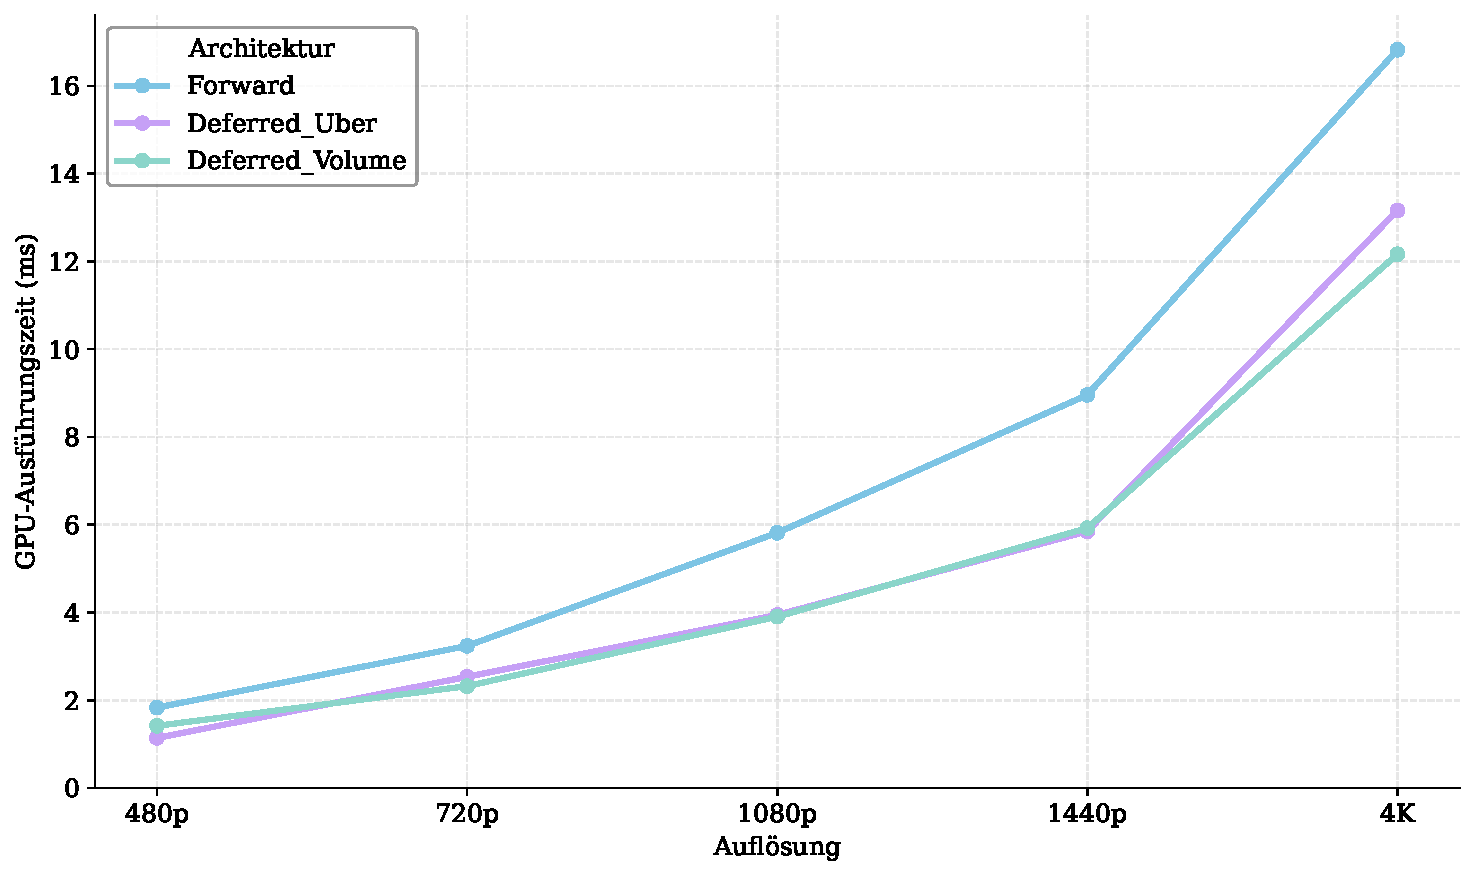
\includegraphics[width=0.85\linewidth]{abbildungen/5_3_1_resolution_scaling_crossover}
    \caption[Messung der GPU-Ausführungszeit bei Auflösungsskalierung]{Messung der GPU-Ausführungszeit in Abhängigkeit von
    der Framebuffer-Auflösung (480p bis 4K) unter einer statischen Last von 200 Lichtquellen.}
    \label{fig:5_3_1_resolution_scaling_crossover}
\end{figure}

% Deduktion.
Die starken Einbußen von Forward gegenüber den Deferred-Pipelines wird im Zusammenhang mit \textit{Shading-Overdraw} vermutet.
Da in diesem Setup $N_{\text{Light}} = 200$ Lichter berechnet werden, führt die Forward-Pipeline komplexe
Beleuchtungsmathematik auf Fragmenten aus, die später von anderen Objekten verdeckt
werden (vgl.\ Kap.~\ref{subsec:020301_overdraw}).
Bei einer Anzahl von $8{,}3\text{ Millionen}$ Pixeln (4K) multipliziert sich diese redundante Rechenlast wesentlich
stärker als bei den entkoppelten Deferred-Pipelines (ein \ac{ALU}-Limit wird schneller erreicht)
~\cite[Abschn.~1]{mallettDeferredAdaptiveCompute2018}.
Diese Vervielfachung der redundanten Rechenlast bei steigender Pixelanzahl stützt die Annahme aus
\hyperlink{hyp:H1.1}{Hypothese H1.1}.

\subsection{{Bandbreiten}}
\label{subsec:050302_bandwidth_eval}

% Einleitung.
Ziel der folgenden Evaluation ist die Isolierung der absoluten Speicherbandbreite (Fillrate) und des Basis-Overheads der
Rendering-Pipelines.
Der Versuchsaufbau gründet auf einem simplen binären Test.
Die Szene ist in diesem Fall vollständig leer ($N_{\text{Inst}} = 0$, $N_{\text{Light}} = 0$).
Es erfolgt lediglich eine Aktivierung bzw.\ Deaktivierung eines vollflächigen Boden-Quads (in 1080p und 4K Auflösung).
Im Rahmen dessen werden die Bandbreiten-Nachteile während des Schreibens und Lesens der Framebuffer
ausgelotet.

% Aufbau.
\begin{center}
    \small
    \colorbox{gray!5}{\parbox{0.95\textwidth}{
        \centering
        \vspace{2mm}
        {\sffamily\bfseries Versuchs-Setup} \\[1.5ex]
        \begin{tabularx}{0.9\textwidth}{>{\sffamily}l X}
            Unabhängige Variablen:   & Sichtbarkeit des Bodens ($C_{\text{Floor}} \in \{\text{Deaktiviert},
            \text{Aktiviert}\}$), Render-Auflösung ($R \in \{1080\text{p}, 4\text{K}\}$) \\
            Metrik (Zustände):       & 0 sichtbare Fragmente vs. $100\,\%$ Screen-Space-Abdeckung
            ($\approx 2\text{ Mio. vs. } \approx 8{,}3\text{ Mio. Pixel}$) \\
            Kontrollvariablen:       & $N_{\text{Inst}} = 0$, $N_{\text{Light}} = 0$ \\
            Zielgröße:               & \ac{GPU}-Gesamtlaufzeit ($t_{\text{GPU}}$)
        \end{tabularx}
        \vspace{2mm}
    }}
\end{center}

% Beobachtungen.
Bei Betrachtung der Abbildung~\ref{fig:5_3_2_1_base_bandwidth_tax_means} lassen sich zwei grundlegende Aspekte
feststellen.
Die Basislast der Deferred-Pipelines scheint im Vergleich zu der Forward-Pipeline geringfügig höher zu sein.
Ansonsten kann keine signifikante prozentuale Steigerung der \ac{GPU}-Aufwände zwischen den Pipelines in der 1080p
Messung festgestellt werden.
Bei der Initialisierung des bildschirmfüllenden Boden-Quads zeigen sowohl die Forward- als auch die beiden
Deferred-Pipelines eine annähernd identische Skalierung, wobei sich die $t_{\text{GPU}}$-Zeit in allen Fällen um etwa
\qty{64}{\percent} erhöht.
Abbildung~\ref{fig:5_3_2_2_base_bandwidth_tax_means} zeigt jedoch, dass die Deferred-Volume-Pipeline bei einer
Auflösung von 4K im Vergleich zu den anderen Single-Pass-Pipelines signifikant schlechter skaliert.

% Ergebnis Graph 1
\begin{figure}[htbp]
    \centering
    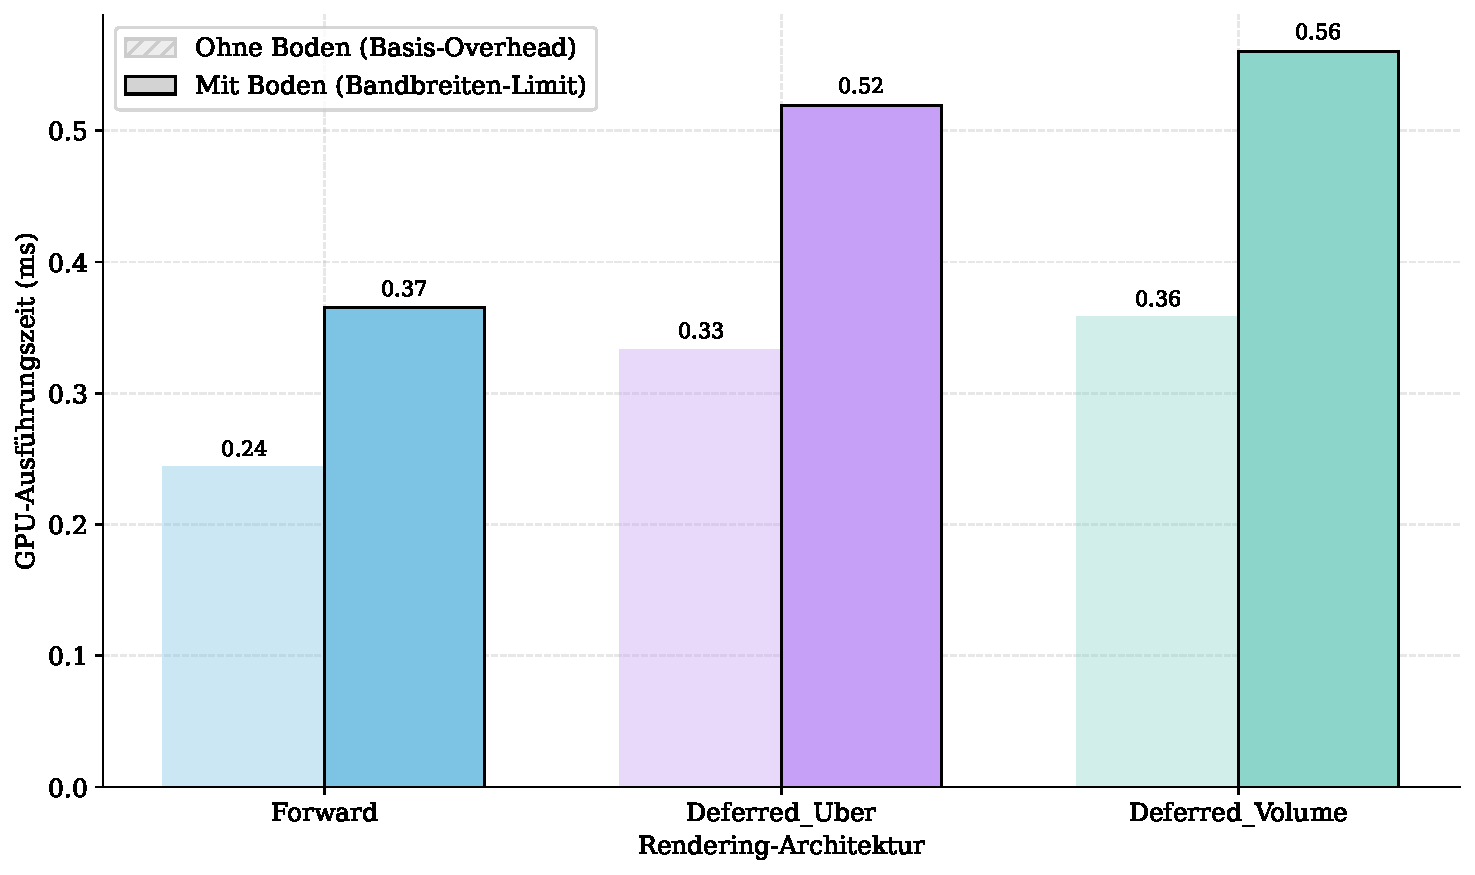
\includegraphics[width=0.85\linewidth]{abbildungen/5-3-2-1_BaseBandwidthTax_Means}
    \caption[Vergleich der Basis-Bandbreitenkosten bei 1080p]{Vergleich der GPU-Ausführungszeit zwischen keiner
    Geometrielast (Basis-Overhead) und vollflächiger Screen-Space-Abdeckung bei 1080p Auflösung ohne Beleuchtung.}
    \label{fig:5_3_2_1_base_bandwidth_tax_means}
\end{figure}

% Ergebnis Graph 1
\begin{figure}[htbp]
    \centering
    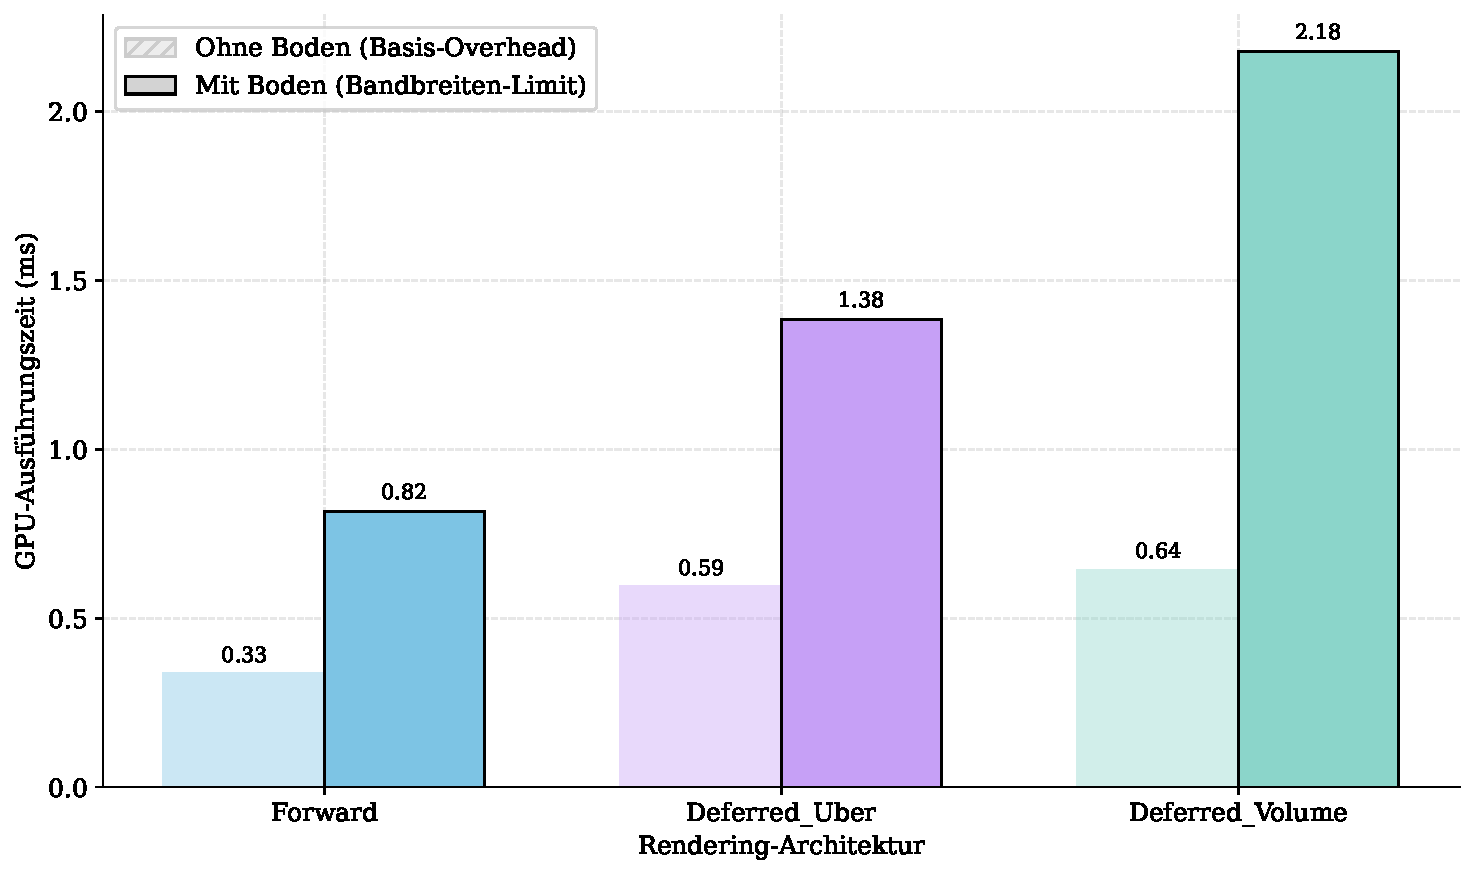
\includegraphics[width=0.85\linewidth]{abbildungen/5-3-2-2_BaseBandwidthTax_Means}
    \caption[Vergleich der Basis-Bandbreitenkosten bei 4K]{Vergleich der GPU-Ausführungszeit zwischen keiner
    Geometrielast (Basis-Overhead) und vollflächiger Screen-Space-Abdeckung bei 4K Auflösung ohne Beleuchtung.}
    \label{fig:5_3_2_2_base_bandwidth_tax_means}
\end{figure}

% Deduktion.
Die Gegenüberstellung der Messreihen bei 1080p und 4K lässt auf einen physischen Hardware-Engpass schließen.
Bei einer Auflösung von 1080p ist die \ac{VRAM}-Bandbreite noch ausreichend, um den Lese- und Schreibverkehr von circa
zwei Millionen Pixeln ohne Verzögerungen abzuwickeln.
Bei einer Vervierfachung der Datenlast, wie sie bei 4K-Auflösungen erreicht wird, kommt es jedoch zur Sättigung des
Speicherbusses.
Wäre die Ursache ein reines Rechenproblem der Shader (\ac{ALU}-Limit), müssten alle Pipelines bei 4K proportional
gleichmäßig skalieren.
Die signifikant stärkere Einbuße der Deferred-Volume-Pipeline bei der 4K-Auflösung (\qty{240}{\percent}) im Vergleich
zu den Forward- und Uber-Shader-Ansätzen (\qty{135}{\percent}) lässt sich primär auf den hardwarenahen Overhead des
additiven Blendings (vgl.\ Kap.~\ref{subsec:020302_memory_bandwidth}) zurückführen und liefert ein starkes Indiz für die
\hyperlink{hyp:H3}{Hypothese H3}.
Deferred-Uber und Forward rechnen das finale Beleuchtungsergebnis in einem einzigen Durchlauf aus
(Single-Pass-Architektur) und überschreiben den Zielpuffer direkt (nur eine Replace-Operation).
Die Multi-Pass-Architektur der Volume-Pipeline hingegen erfordert zwingend den kontinuierlichen Einsatz von additivem
Blending zur Akkumulation der Lichtbeiträge~\cite[S.~9]{lauritzenDeferredRenderingCurrent}.
\textcite[S.~803]{akenine-mollerRealtimeRendering2019} weisen darauf hin, dass derartige Blending-Operationen auf dem
\ac{VRAM}-Bus im Vergleich zu einfachen Schreibvorgängen mit signifikant höheren Kosten verbunden sind.
In Kombination mit dem simultanen Auslesen der breiten \ac{G-Buffer} resultiert dieser zusätzliche
Lese-Schreib-Zyklus bei $8{,}3\,\text{Millionen}$ Pixeln (4K) selbst bei simplen Ambient-Auswertungen
($N_{\text{Light}} = 0$) in einer Sättigung der Speicherbandbreite.

% Limits
Trotz dieser starken theoretischen Indizien muss an dieser Stelle eine methodische Einschränkung des entwickelten
Frameworks eingeräumt werden.
Da die Testumgebung primär auf die Messung von Ausführungszeiten ausgelegt ist, fehlen native
Schnittstellen zur direkten Auslesung spezifischer Hardware-Counter der \ac{GPU}, wie beispielsweise der expliziten
Bus-Auslastung.
In dieser Evaluation im Besonderen kann die tatsächliche Ursache für den Leistungsabfall der
Deferred-Volume-Pipeline somit nicht zweifelsfrei geklärt werden.
Die präzise Evaluierung von Bandbreiten- und Bus-Limitierungen verbleibt daher als eine architektonische Schwäche der
vorliegenden Testarchitektur.


\section{{Beleuchtung}}
\label{sec:0504_lighting_eval}

Im nachfolgenden Abschnitt werden Benchmarks und Erkenntnisse präsentiert, die dazu dienen, die beleuchtungsspezifischen
Limitierungen zu ermitteln.
Da Deferred Rendering im Bereich der Beleuchtungsberechnung signifikante Vorteile verspricht, sollen im Folgenden die
genauen architektonischen Crossover-Points ermittelt werden, ab denen die Deferred-Pipelines die Forward-Pipelines
übertreffen.
Auf Hardware-Ebene werden im Rahmen der vorliegenden Untersuchung die \ac{ALU}- und \ac{ROP}-Limits mithilfe der nachfolgenden
Benchmarks evaluiert.

\subsection{{Lichtanzahl}}
\label{subsec:050401_light_count_eval}

% Einführung.
Ziel dieser Evaluation ist die Untersuchung der Skalierbarkeit von Punktlichtern.
Dazu wird der klassische Ansatz der \ac{UBO}-Iteration (Forward und Deferred-Uber) mit der Rasterisierung von
Proxy-Geometrie (Deferred-Volume) verglichen.
Die Anzahl der Lichtquellen $N_{\text{Light}}$ wird dabei logarithmisch von $10$ auf bis zu $5.000$ skaliert.
Wie in Unterkapitel Kapitel~\ref{subsec:040201_forward_pipeline} beschrieben, sind sowohl die Forward-Pipeline
als auch die Deferred-Uber-Pipeline hinsichtlich der maximal nutzbaren Lichtquellen durch die
\ac{UBO}-Limits auf insgesamt 500 Punktlichter limitiert.
Im Rahmen der Untersuchung der allgemeinen Skalierung erfolgt zudem eine Evaluation der Deferred-Volume-Pipeline mit bis
zu $5.000$ Lichtquellen.
Darüber hinaus zeichnet sich das szenische Setup durch eine minimale Überlappung der Lichtquellen und deren Radien
aus um Blending-Operationen möglichst gering zu halten.

% Aufbau.
\begin{center}
    \small
    \colorbox{gray!5}{\parbox{0.95\textwidth}{
        \centering
        \vspace{2mm}
        {\sffamily\bfseries Versuchs-Setup} \\[1.5ex]
        \begin{tabularx}{0.9\textwidth}{>{\sffamily}l X}
            Unabhängige Variable:    & Anzahl aktiver Lichtquellen ($N_{\text{Light}} \in \{10, \dots, 5.000\}$) \\
            Kontrollvariablen: & Umgebungslicht deaktiviert ($I_{\text{Ambient}} = 0{,}0$), Licht-Radius
            reduziert ($r_{\text{Light}} = 1{,}0$) \\
            Architektonische Limits:   & Forward und Deferred-Uber limitiert auf max.\ 500 Lichter
            (\ac{UBO}-Limit) \\
            Zielgröße:               & \ac{GPU}-Gesamtlaufzeit ($t_{\text{GPU}}$)
        \end{tabularx}
        \vspace{2mm}
    }}
\end{center}

% Beschreibung.
Die Ergebnisse, dargestellt in Abbildung~\ref{fig:5_4_1_light_count_means}, zeigen eine nahezu identische Verteilung der
Pipelines bei einer Lichtanzahl von $\le 50$ Punktlichtern.
Bei geringer Last nimmt die Forward-Pipeline eine leicht überlegene Position ein.
Bei einer Last von etwa 100 Lichtquellen lässt sich allerdings ein Kipppunkt zugunsten beider Deferred-Pipelines
erkennen.
Obwohl die Deferred-Uber-Pipeline eine signifikant geringere Skalierbarkeit aufweist als die
Deferred-Volume-Pipeline, übertrifft diese ab dem 100-Lichter-Kipppunkt die Forward-Pipeline zunehmend,
wenn auch nur marginal.
Bei einer Anzahl von 250 Lichtquellen zeigt sich ein signifikanter Einbruch der Leistung von Forward, während
Deferred-Volume eine extreme Effizienz und flache Skalierung aufweist.
Erst bei einer Last von $5.000$ Lichtquellen überschreitet die Deferred-Volume-Pipeline die Rechenzeit von
Forward bei einer zehnmal geringeren Last von 500 Lichtern.

% Ergebnis Graph.
\begin{figure}[htbp]
    \centering
    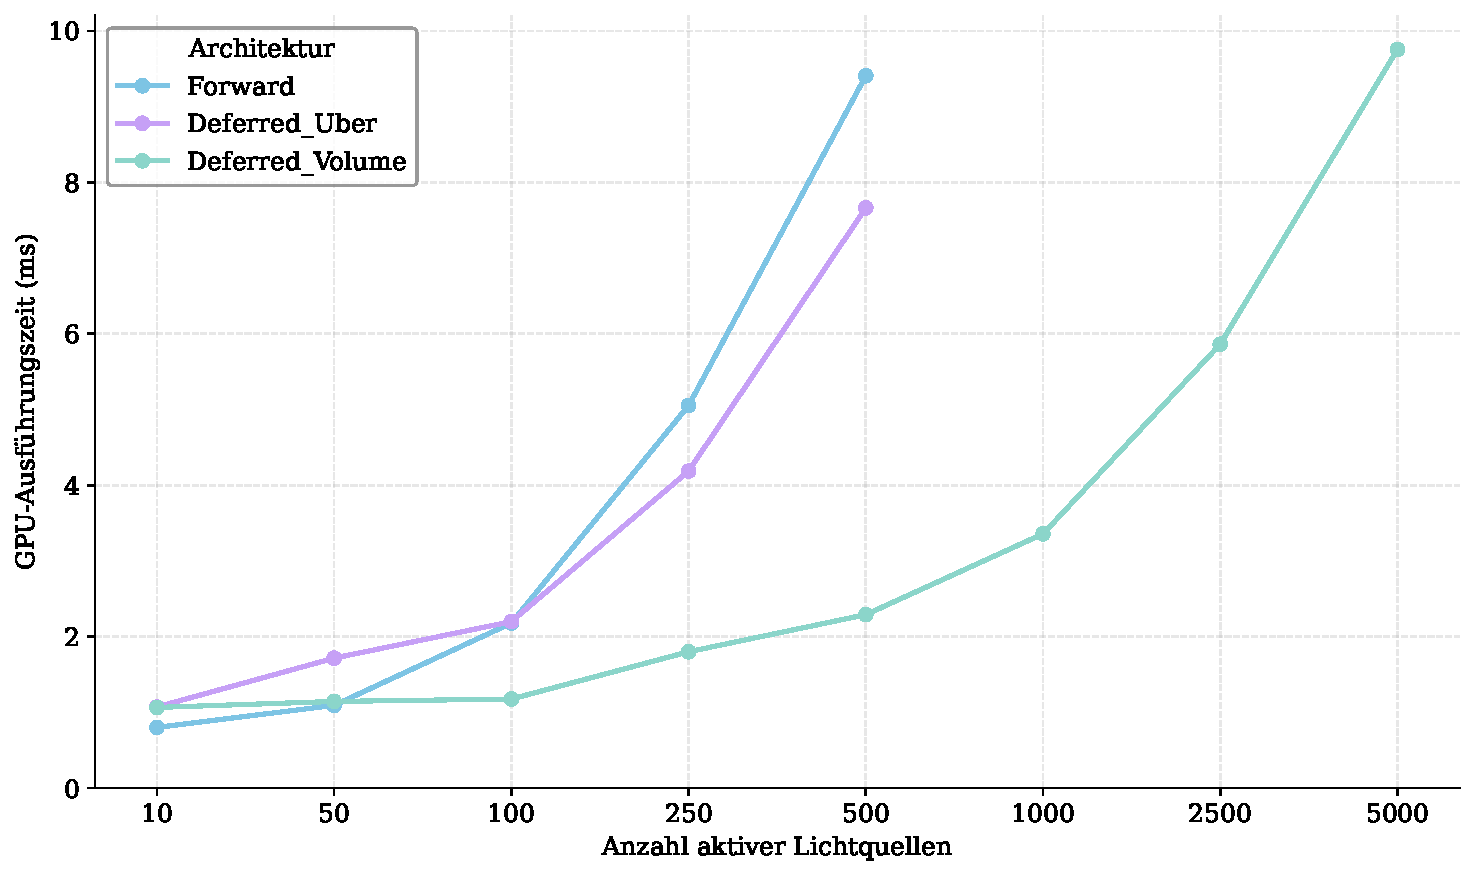
\includegraphics[width=0.85\linewidth]{abbildungen/5-4-1_LightCount_Means}
    \caption[Messung der GPU-Ausführungszeit bei Lichtanzahlskalierung]
    {Messung der GPU-Ausführungszeit in Abhängigkeit
    von der Anzahl aktiver Lichtquellen (10 bis 5.000).}
    \label{fig:5_4_1_light_count_means}
\end{figure}

% Deduktion
Aus den Beobachtungen kann abgeleitet werden, dass die Deferred-Pipelines bei steigender Lichtanzahl grundlegend besser
skalieren als einfache Forward-Ansätze.
Diese Erkenntnis validiert die in der Literatur beschriebene Überlegenheit von Deferred-Rendering im Bereich massiver
Lichtevaluationen und bestätigt den primären Existenzgrund dieses Paradigmas im
Allgemeinen~\cite[S.~1]{Thaler2011DeferredRendering}.
Obwohl die Deferred-Uber-Pipeline den gleichen Loop zur Beleuchtungsberechnung ausführt wie der Forward-Ansatz, wird
durch das Entkoppeln der Geometrie der Shading-Overdraw effektiv vermieden.
Der Einsatz des \ac{G-Buffer}s gewährleistet, dass die Schleife für die Lichtberechnung lediglich für die auf dem
Bildschirm tatsächlich sichtbaren Pixel ausgeführt wird.
Die signifikante Überlegenheit des Deferred-Volume-Ansatzes lässt sich auf die Effizienz des lokal begrenzten
Evaluationsbereiches der Licht-Volumes zurückführen.
Anstelle eines volumenunabhängigen Vollbild-Passes wird seitens der \ac{GPU} lediglich eine Rasterisierung der
Licht-Proxy-Geometrien vorgenommen.
Die \ac{ALU}-Last beschränkt sich somit exakt auf die Screen-Space-Projektion, in der das Lichtvolumen die Geometrie
tatsächlich beeinflusst~\cite[S.~886]{akenine-mollerRealtimeRendering2019}.
Bei einer extremen Last von $5.000$ Lichtquellen lässt sich zudem die Hypothese aufstellen, dass das Limit der
Deferred-Volume-Pipeline primär durch die \ac{VRAM}-Bandbreite der \ac{ROP}s aufgrund des massiven
\textit{Read-Modify-Write}-Zyklus des additiven Blendings erreicht wird
(siehe Kapitel~\ref{subsec:050302_bandwidth_eval}).
Diese Beobachtung verifiziert den algorithmischen Kern von \hyperlink{hyp:H1.1}{Hypothese H1.1}: Die multiplikative
Komplexität der direkten Beleuchtungsberechnung zwingt die Forward-Architektur bei steigender Lichtkomplexität unweigerlich
in ein massives Performance-Defizit.

\subsection{{Lichtintensität \& Overlap}}
\label{subsec:050402_light_intensity_and_overlap_eval}

% Einleitung.
Ziel der folgenden Untersuchungen ist die Evaluation der Pipelines unter Bedingungen extremer räumlicher Dichte der
Lichtquellen und des damit verbundenen massiven \textit{Light Overdraws}.
Es werden zwei komplementäre Szenarien evaluiert: Test A skaliert den physikalischen Radius von 250 Lichtquellen, um die
Bildschirmabdeckung künstlich in die Höhe zu treiben, während Test B bis zu $1.000$ Lichtquellen auf exakt dieselbe
3D-Koordinate (Singularität) zwingt, um eine maximale Überlagerung pro Pixel zu garantieren.
Dieses Versuchsdesign verspricht die gezielte Provokation und Isolierung des
\textit{Read-Modify-Write}-Bandbreitenlimits der Rasterisierungseinheiten (\acp{ROP}).
Es soll aufgezeigt werden, an welchem Punkt die kontinuierliche Speicher-Akkumulation bei überlappenden Lichtvolumina
die reine \ac{ALU}-Rechenlast der Shader-Schleifen als primärer Performance-Flaschenhals ablöst.

% Aufbau.
\begin{center}
    \small
    \colorbox{gray!5}{\parbox{0.95\textwidth}{
        \centering
        \vspace{2mm}
        {\sffamily\bfseries Versuchs-Setup} \\[1.5ex]
        \begin{tabularx}{0.9\textwidth}{>{\sffamily}l X}
            \multicolumn{2}{l}{\textbf{Test A: Skalierung der Lichtintensität (Radius)}} \\
            Unabhängige Variable:    & Licht-Radius-Multiplikator ($r_{\text{Light}} \in \{0{,}5, \dots, 20{,}0\}$) \\
            Kontrollvariablen:& $N_{\text{Light}} = 250$ (fixiert), Umgebungslicht deaktiviert
            ($I_{\text{Ambient}} = 0{,}0$) \\[1.5ex]

            \multicolumn{2}{l}{\textbf{Test B: Licht-Singularität (Räumliche Ballung)}} \\
            Unabhängige Variable:    & Anzahl aktiver Lichtquellen ($N_{\text{Light}} \in \{10, \dots, 1.000\}$) \\
            Kontrollvariablen:& Licht-Singularität aktiviert ($S_{\text{Light}} = \text{Aktiviert}$),
            $I_{\text{Ambient}} = 0{,}0$ \\[1.5ex]

            Zielgröße:               & \ac{GPU}-Gesamtlaufzeit ($t_{\text{GPU}}$)
        \end{tabularx}
        \vspace{2mm}
    }}
\end{center}

% Beobachtung.
Die Analyse der Abbildung~\ref{fig:5_4_2_1_light_intensity_means} zeigt, dass die Deferred-Volume-Pipeline bei
einem kleinen Radius von $0{,}5$ und dem damit verbundenen minimalen Volume-Overlap den signifikant schnellsten Ansatz
darstellt.
Wird der Radius-Multiplikator auf $20{,}0$ erhört und damit die Screen-Space-Abdeckung drastisch gesteigert, führt dies
zu einer massiven Zunahme der Laufzeit der Deferred-Volume-Pipeline auf über \qty{8}{\milli\second}, während die Werte
für Forward und Deferred-Uber nahezu konstant bleiben.
In Abbildung~\ref{fig:5_4_2_2_light_singularity_means} wird ein identisches Bild in forcierter Form dargestellt.
Die Deferred-Volume-Pipeline bricht bei einer Skalierung auf bis zu $1.000$ Lichtquellen stark ein und
erreicht eine \ac{GPU}-Laufzeit von nahezu \qty{37}{\milli\second}.
Die Deferred-Uber-Pipeline und der Forward-Ansatz zeigen demgegenüber bei einer Auslastung von bis zu 500
Lichtquellen eine signifikant höhere Effizienz und verbleiben stabil unterhalb der \qty{12}{\milli\second}-Marke.

\begin{figure}[htbp]
    \centering
    
\includegraphics[width=0.85\linewidth]{abbildungen/5-4-2-1_LightIntensity_Means}
    \caption[Messung der GPU-Ausführungszeit bei Lichtintensitätsskalierung]{Messung der GPU-Ausführungszeit in Abhängigkeit
    von der Lichtintensität respektive dem Radius-Multiplikator (0,5 bis 20,0) bei einer konstanten Anzahl von 250
    Lichtquellen.}
    \label{fig:5_4_2_1_light_intensity_means}
\end{figure}

\begin{figure}[htbp]
    \centering
    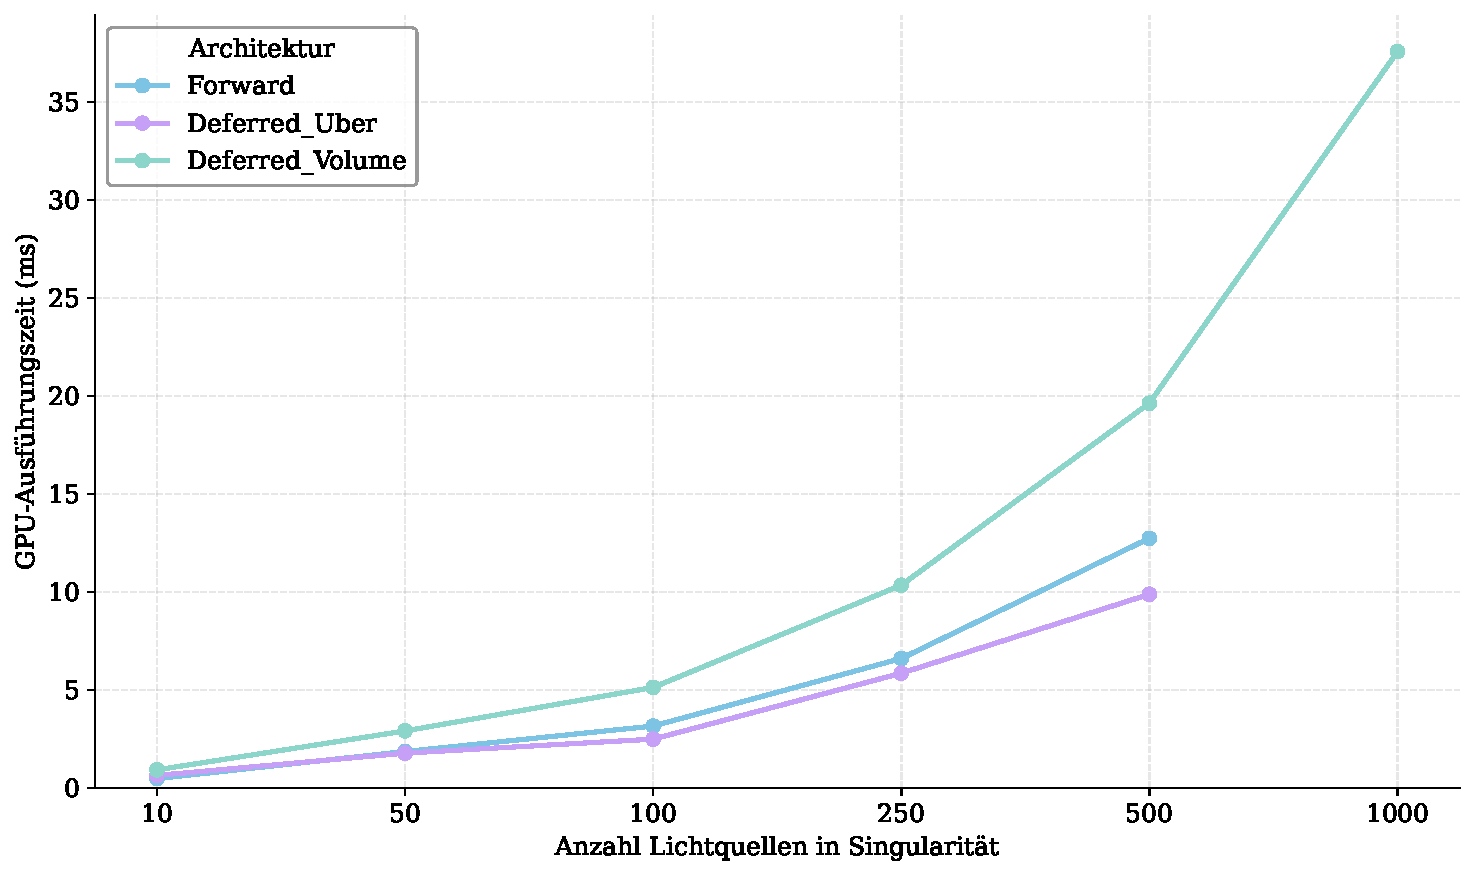
\includegraphics[width=0.85\linewidth]{abbildungen/5-4-2-2_LightSingularity_Means}
    \caption[Messung der GPU-Ausführungszeit bei Lichtquellen-Singularität]{Messung der GPU-Ausführungszeit in Abhängigkeit von der
    Anzahl der Lichtquellen (10 bis 1000) bei einer Positionierung aller Lichtquellen in einer räumlichen Singularität.}
    \label{fig:5_4_2_2_light_singularity_means}
\end{figure}

% Deduktion
Diese Untersuchungen forcieren die in den Kapiteln~\ref{subsec:050302_bandwidth_eval}
und~\ref{subsec:050401_light_count_eval} beobachteten Phänomene im Zusammenhang mit den \ac{ROP}- und Bandbreitenlimits
der Deferred-Volume-Pipeline und verifizieren \hyperlink{hyp:H3}{Hypothese H3} abschließend:
Sie verorten die größte architektonische Limitierung des Deferred-Volume-Ansatzes in Szenarien mit hochgradig
überlappenden Einflussbereichen verschiedener Lichtquellen.
Wenn hunderte Licht-Volumina dieselbe Pixelfläche abdecken, zwingt die Deferred-Volume-Pipeline die \ac{GPU},
für diese einzelnen Pixel hunderte Male den \ac{RMW}-Zyklus für das additive Blending (\ac{ROP}s) auf dem Speicherbus
auszuführen~\cites[Folie~9]{lauritzenDeferredRenderingCurrent}[S.~676]{gregoryGameEngineArchitecture2018}
(vgl.\ Kap.~\ref{subsec:020302_memory_bandwidth}).
Der \ac{VRAM}-Speicherbus kollabiert in der Folge unter der schieren Frequenz dieser redundanten Lese- und
Schreibzugriffe.

\subsection{{Shading Overdraw}}
\label{subsec:050403_shading_overdraw_eval}

% Einleitung.
Wie in Unterkapitel~\ref{subsec:050203_overdraw_eval} bereits für die reine Geometrie evaluiert, wird im Folgenden
erneut der Einfluss des Overdraws untersucht.
In diesem Versuchsaufbau wird die Tiefenkomplexität allerdings unter Zuhilfenahme einer konstanten Beleuchtungslast
überprüft.
Der Aufbau ist hierbei nahezu identisch zu~\ref{subsec:050203_overdraw_eval}, mit der Ausnahme von $100$
zusätzlich aktiven Lichtquellen.
Die Anzahl der Lichtquellen ist dabei so gewählt, dass sie den in
Kapitel~\ref{subsec:050402_light_intensity_and_overlap_eval} aufgezeigten \textit{Light-Volume-Overlap} innerhalb der
Deferred-Volume-Pipeline möglichst geringfügig provoziert.
Für die Messergebnisse wird erwartet, dass der Forward-Ansatz durch klassischen Shading-Overdraw an Effizienz verliert,
da die aufwendige Beleuchtungsberechnung hier untrennbar mit der Geometrieauswertung verknüpft ist
(vgl.\ Kap.~\ref{subsec:020201_forward_rendering}).
Somit sollte sich der Berechnungsaufwand theoretisch mit jedem überzeichneten Fragment vervielfachen
(vgl.\ Kap.~\ref{subsec:020301_overdraw}).

% Aufbau
\begin{center}
    \small
    \colorbox{gray!5}{\parbox{0.95\textwidth}{
        \centering
        \vspace{2mm}
        {\sffamily\bfseries Versuchs-Setup} \\[1.5ex]
        \begin{tabularx}{0.9\textwidth}{>{\sffamily}l X}
            Unabhängige Variable:    & Instanzanzahl ($N_{\text{Inst}} \in \{2.000, \dots, 32.000\}$) \\
            Kontrollvariablen:       & $N_{\text{Light}} = 100$, Spawn-Radius reduziert ($r_{\text{Spawn}} = 30{,}0$),
            Boden deaktiviert ($C_{\text{Floor}} = \text{Deaktiviert}$) \\
            Metrik (X-Achse):        & Theoretischer Overdraw-Faktor ($\approx 1{,}1$ bis $18{,}1$) \\
            Zielgröße:               & \ac{GPU}-Laufzeit ($t_{\text{GPU}}$), aufgeschlüsselt nach Komponenten
        \end{tabularx}
        \vspace{2mm}
    }}
\end{center}

% Beschreibung
Abbildung~\ref{fig:5_4_3_decoupling_proof} zeigt, dass der vorgelagerte \ac{G-Buffer}-Pass der Deferred-Pipelines in
diesem Kontext den primären weitestgehend linearen Skalierungsfaktor bei einer ansteigenden Instanzdichte für die beiden
Deferred-Pipelines darstellt.
In der Betrachtung der Forward-Pipeline-Renderzeit ist ein Anstieg der kombinierten Zeit zu verzeichnen
(von \qty{1,11}{\milli\second} auf \qty{5,98}{\milli\second}), der jedoch nicht so stark ausfällt, wie es die
ursprüngliche Annahme vermuten ließe.
Der Engine Overhead weist zudem bei sämtlichen Pipelines eine hohe Konstanz auf.

% Ergebnis Graph.
\begin{figure}[htbp]
    \centering
    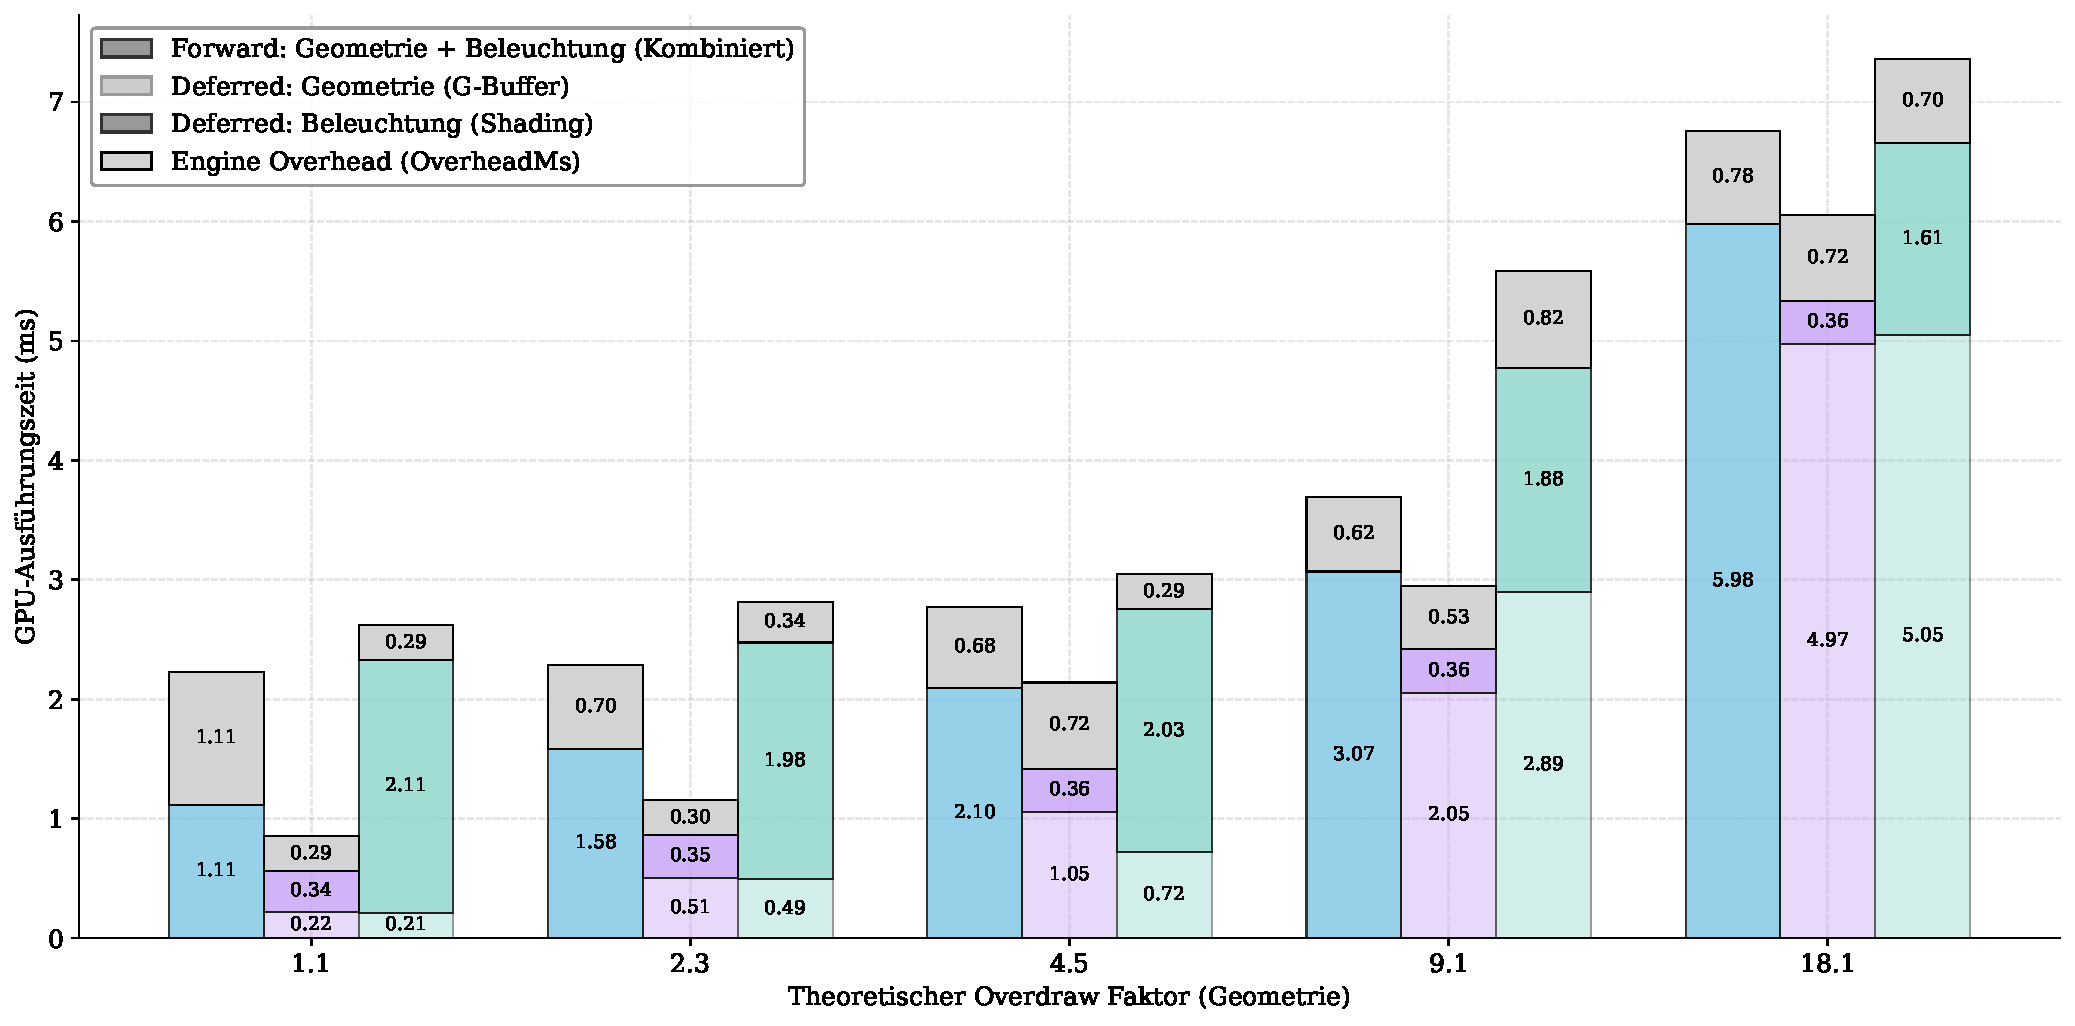
\includegraphics[width=0.85\linewidth]{abbildungen/5_4_3_decoupling_proof}
    \caption[Entkopplungsnachweis in steigendem geometrischen Overdraw]{Aufschlüsselung der GPU-Ausführungszeit nach
    einzelnen Pipeline-Komponenten in Abhängigkeit vom theoretischen Overdraw-Faktor bei einer konstanten Last von 100
    Lichtquellen.}
    \label{fig:5_4_3_decoupling_proof}
\end{figure}

% Deduktion
Die Ergebnisse dieser Evaluation widerlegen die weit verbreitete Annahme, dass der Overdraw, insbesondere in
Kombination mit Beleuchtung, in einfachen Forward-Pipelines einen der größten Engpässe
darstellt~\cites[Abschn.~1]{Thaler2011DeferredRendering}.
Die Ergebnisse dieser Evaluation erzwingen somit eine Relativierung der \hyperlink{hyp:H1.1}{Hypothese H1.1}:
Durch hardwarebasierte Optimierungen wie \textit{Early-Z} wird auf modernen Grafikkarten auch ohne dedizierten,
softwarebasierten \textit{Z-Prepass} ein signifikanter Teil der redundanten Rechenlast der Beleuchtungsberechnung
verdeckter Fragmente vermieden~\cite[S.~801~u.~803]{akenine-mollerRealtimeRendering2019} (vgl.\ Kap.~\ref{subsec:020301_overdraw}).


\section{{Hybride Stilisierung \& Entropie}}
\label{sec:0505_npr_eval}

In den vorangegangenen Untersuchungskapiteln wurde das grundlegende Verhalten der evaluierten Rendering-Architekturen
aufgezeigt und somit zugleich die Fähigkeiten und Grenzen des \ac{HyDra}-Frameworks demonstriert.
Die nachfolgenden Tests widmen sich dem Kern der Forschung und evaluieren die Wechselwirkungen von Stil-Entropie und
den allgemeinen Einfluss selektiver \ac{NPR}-Techniken auf die verschiedenen Pipelines.
Der Fokus liegt hierbei, im Speziellen auf der Evaluation von Warp Divergence und Registerdruck.

\subsection{{Stil-Entropie}}
\label{subsec:050501_entropy_eval}

% Einleitung.
In den nachfolgenden, zusammengefassten Versuchen werden die Einflüsse von stilistischer Komplexität mittels der
Anwendung diverser \ac{NPR}-Stile analysiert.
Neben dem bisher standardmäßig verwendeten Blinn-Phong-Shading finden auch Toon-Shading und Gooch-Shading
Anwendung (vgl\ Kap.~\ref{sec:0403_npr_payloads}).
In der vorliegenden Untersuchung \textit{A} wird eine sortierte (niedrige Entropie) mit einer gestreuten (hohe
Entropie) Objektverteilung verglichen, wobei die Anzahl der Stile konstant bei drei bleibt.
In der weiteren Untersuchung \textit{B} wird die Anzahl der simultan aktiven Shading-Stile von 1 bis 3 (Blinn, Gooch,
Toon) skaliert.
In diesem verteilten Szenario (Versuch \textit{B}) führt die schrittweise Zunahme der Stile zudem zur Isolation des
algorithmischen Einflusses der \ac{NPR}-Effekte.
Die vorliegende Untersuchung zielt darauf ab, die Hypothesen der Warp-Divergenz und des Registerdrucks zu analysieren
und zu verifizieren.
Diese Analyse erfolgt vornehmlich mit Blick auf die Performance der Deferred-Uber-Pipeline.

% Aufbau.
\begin{center}
    \small
    \colorbox{gray!5}{\parbox{0.95\textwidth}{
        \centering
        \vspace{2mm}
        {\sffamily\bfseries Versuchs-Setup} \\[1.5ex]
        \begin{tabularx}{0.9\textwidth}{>{\sffamily}l X}
            \multicolumn{2}{l}{\textbf{Versuch A: Räumliche Entropie}} \\
            Unabhängige Variable:    & Räumliche Verteilung ($E_{\text{Spatial}} \in \{\text{Sortiert},
            \text{Gestreut}\}$) \\
            Kontrollvariablen:& $N_{\text{Inst}} = 15.000$, $N_{\text{Light}} = 250$,
            $r_{\text{Spawn}} = 175{,}0$, Drei aktive Stile ($S_{\text{Count}} = 3$) \\[1.5ex]

            \multicolumn{2}{l}{\textbf{Versuch B: Kombinatorische Degradation}} \\
            Unabhängige Variable:    & Anzahl aktiver Rendering-Stile ($S_{\text{Count}} \in \{1, 2, 3\}$) \\
            Kontrollvariablen:       & Gleicher Aufbau wie Test A, Räumliche Entropie geklustert
            ($E_{\text{Spatial}} = \text{Geklustert}$) \\[1.5ex]

            Zielgröße:               & \ac{GPU}-Beleuchtungs-Zeit ($t_{\text{Light}}$)
        \end{tabularx}
        \vspace{2mm}
    }}
\end{center}

% Beschreibung.
In beiden Ergebnisgraphen (siehe Abbildung~\ref{fig:5_5_1_entropy_divergence_means}
\&~\ref{fig:5_5_2_style_combinatorics_gpu}) ist zu erkennen, dass sowohl Forward als auch Deferred-Volume
bei gestreuter Verteilung der Stile (hohe Entropie) im Vergleich zu sortierten Verhältnissen extrem stabil bleiben.
Auch der erhöhte algorithmische Aufwand in der Lichtberechnung, der durch die komplexeren Aufwände der Toon- und
Gooch-Shader entsteht, zeigt nur minimalen Einfluss auf Forward- und Deferred-Volume.
Die Deferred-Uber-Pipeline weist in beiden Szenarien allerdings einen signifikanten Einbruch auf und
verdoppelt nahezu ihren Aufwand (Anstieg der Beleuchtungsberechnungs-Zeiten um $\approx$\,\qty{85}{\percent}) bei
einer gestreuten Stil-Verteilung (hohe Entropie).
Abbildung~\ref{fig:5_5_1_entropy_divergence_means_live_hydra} zeigt den Versuchsaufbau innerhalb des \textit{HyDra}
Frameworks.

\begin{figure}[htbp]
    \centering
    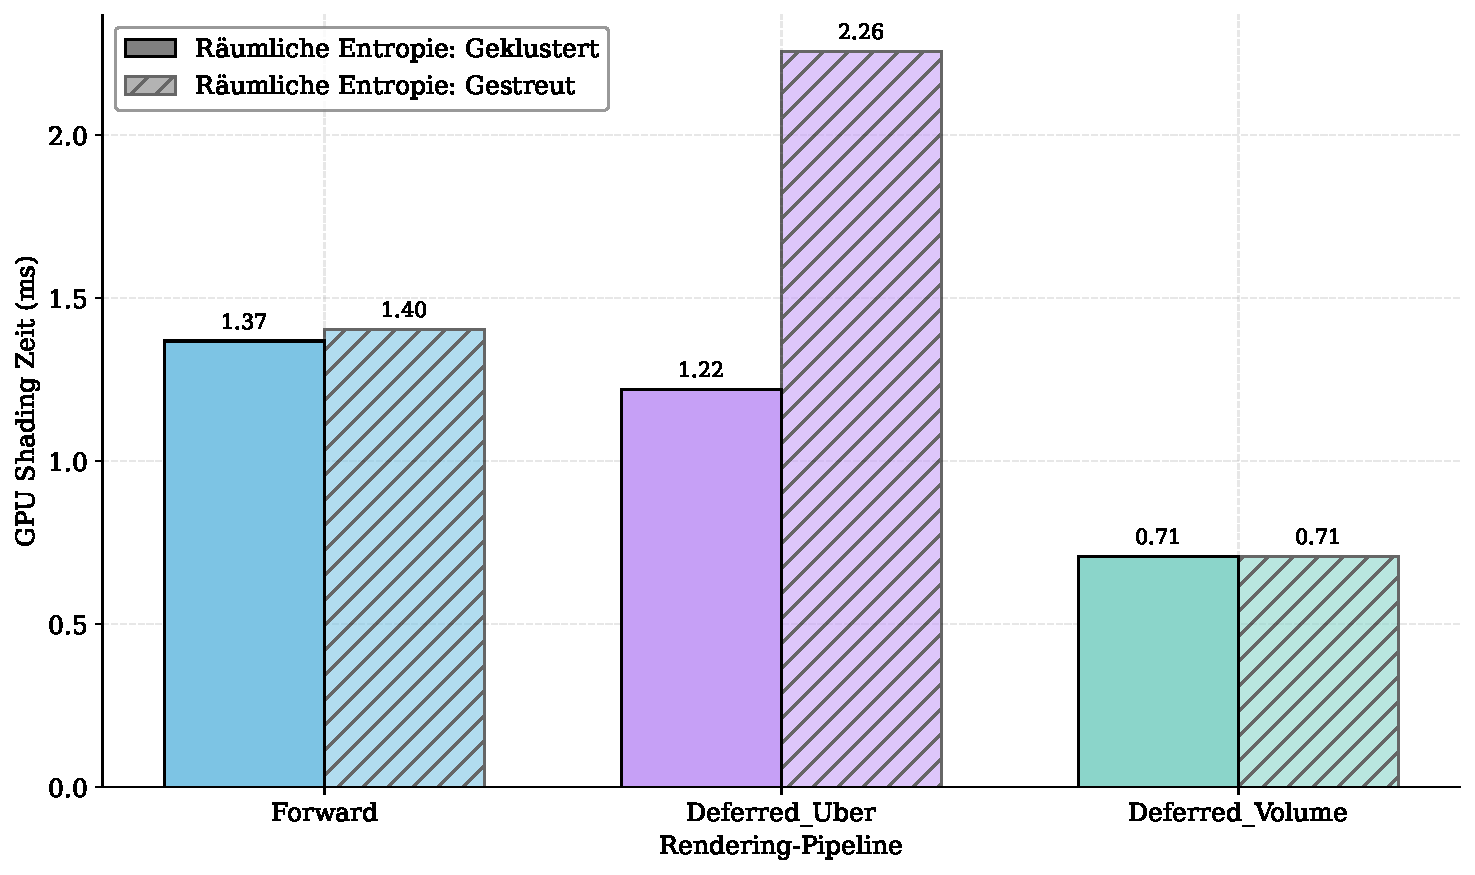
\includegraphics[width=0.85\linewidth]{abbildungen/5_5_1_entropy_divergence_means}
    \caption[Messung der GPU-Shading-Zeit bei variierender Stilverteilung]{Messung der GPU-Shading-Zeit in Abhängigkeit von
    der räumlichen Verteilung (sortiert vs.~gestreut) der Rendering-Stile.}
    \label{fig:5_5_1_entropy_divergence_means}
\end{figure}

% Abbildung aus Engine.
\begin{figure}[htbp]
    \centering
    % Linkes Bild
    \begin{subfigure}[b]{0.49\textwidth}
        \centering
        
\includegraphics[width=0.85\linewidth]{abbildungen/hydra_capture_20260628_110904}
        \caption{Sortierte Verteilung}
        \label{fig:hydra_quadrants}
    \end{subfigure}
    \hfill
    % Rechtes Bild
    \begin{subfigure}[b]{0.49\textwidth}
        \centering
        
\includegraphics[width=0.85\linewidth]{abbildungen/hydra_capture_20260628_110909}
        \caption{Gestreute Verteilung}
        \label{fig:hydra_random}
    \end{subfigure}
    \caption[Vergleich der Stil-Entropie-Verteilungen in HyDra-Framework]{Vergleich der Stil-Entropie Verteilungen in HyDra-Framework während der 5.5.1 Test-Suite in Test A
        (räumliche Entropie).}
    \label{fig:5_5_1_entropy_divergence_means_live_hydra}
\end{figure}

\begin{figure}[htbp]
    \centering
    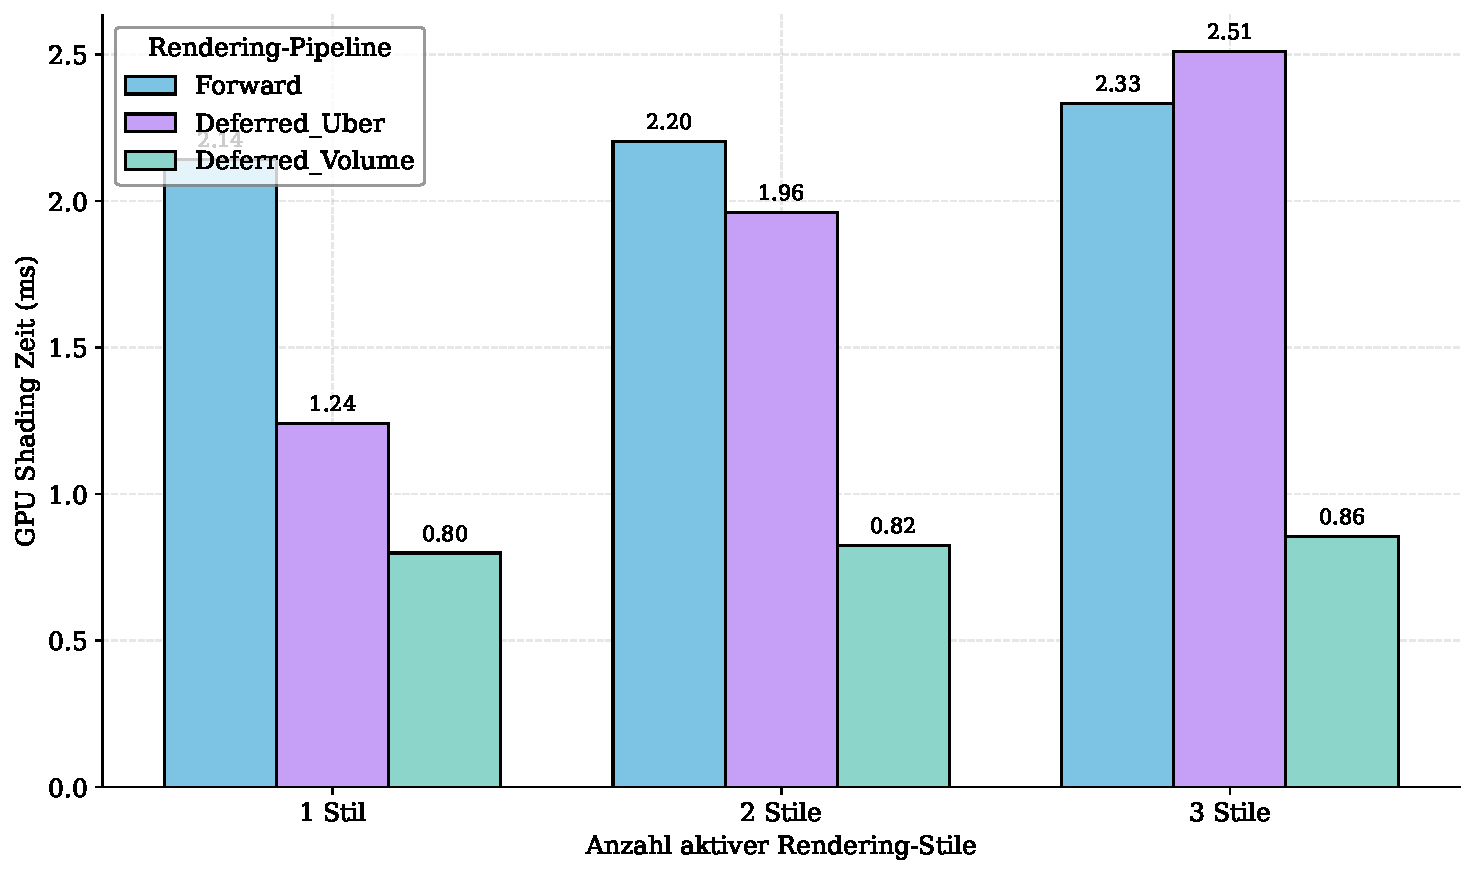
\includegraphics[width=0.85\linewidth]{abbildungen/5_5_2_style_combinatorics_gpu}
    \caption[Messung der GPU-Shading-Zeit bei stilistischer Kombinatorik]{Messung der GPU-Shading-Zeit in Abhängigkeit
    von der Anzahl simultan aktiver Rendering-Stile (1 bis 3 Stile).}
    \label{fig:5_5_2_style_combinatorics_gpu}
\end{figure}

% Deduktion.
In den theoretischen Grundlagen in Kapitel~\ref{subsec:020303_warp_divergence_and_register_pressure} wurde
dargelegt, dass die \ac{GPU} Instruktionen im \ac{SIMT}-Verfahren in sogenannten \textit{Warps} verarbeitet.
Der signifikante Leistungseinbruch der Deferred-Uber-Pipeline im gestreuten Szenario stellt die praktische
Manifestation der \textit{Warp Divergence} dar und verifiziert \hyperlink{hyp:H2}{Hypothese H2} vollumfänglich.
Da benachbarte Pixel innerhalb eines Warps unterschiedliche Shading-Modelle evaluieren, wird die Hardware durch diese
räumliche Entropie dazu gezwungen, die divergierenden Code-Pfade sequenziell abzuarbeiten.
Die Forward- und Deferred-Volume-Architekturen hingegen erweisen sich als systembedingt immun gegen diesen
architektonischen Engpass.
Die strikte Trennung der \textit{Draw-Calls} nach Material (Forward) oder die Nutzung von mehreren insgesamt
kleineren Shader-Pässen (Deferred-Volume) gewährleistet eine Homogenität der aktiven
Warps~\cite[S.~886]{akenine-mollerRealtimeRendering2019}.

% Register Pressure und Limits.
In Bezug auf die lineare Degradation des Deferred-Shaders bei der Kombination mehrerer Stile lässt sich die
zusätzliche Hypothese eines erhöhten Registerdrucks aufstellen.
Die Implementierung eines zusätzlichen Rendering-Stils im monolithischen Code-Pfad bedingt potenziell die Allokation
weiterer Register pro Thread.

% Einschränkungen.
An dieser Stelle ist jedoch eine methodische Limitierung der vorliegenden Testarchitektur zu berücksichtigen.
Aufgrund der Tatsache, dass die Messung der isolierten Beleuchtungs-Laufzeit ($t_{\text{Light}}$) keine
Low-Level-Telemetriedaten liefert, kann diese spezifische Ursache nicht abschließend empirisch verifiziert werden.
Ohne den Einsatz dedizierter Hardware-Profiler lässt sich nicht zweifelsfrei differenzieren, inwieweit ein erhöhter
Registerdruck zum Leistungsabfall der Deferred-Uber-Pipeline beiträgt.

\subsection{{Kernel Bandbreiten Limits}}
\label{subsec:050502_kernel_eval}

% Einleitung.
Der folgende Versuch fokussiert sich ausschließlich auf die Deferred-Pipelines (Deferred-Uber und Deferred-Volume).
Die vorliegende Untersuchung widmet sich der Analyse der Einflüsse kernelbasierter \ac{NPR}-Effekte.
Durch die Tatsache, dass solche kernelbasierten Effekte in der Forward-Pipeline auf Objektebene nicht realistisch
anwendbar sind (vgl.\\ Kapitel~\ref{subsec:040201_forward_pipeline}) und nur auf gesamter Screen-Space-Ebene anwendbar
sind, kann keine Zielbild-Parität erreicht werden.
Ein aussagekräftiger Vergleich mit den Deferred-Pipelines ist somit nicht möglich.
Für die nachfolgende Evaluation wird der implementierte Kuwahara-Filter herangezogen.
Der Suchradius ($R$) des stilisierenden Kuwahara-Filters wird sukzessive von 2 auf bis zu 16 Pixel erweitert.
Da der Filter im zweidimensionalen Raum agiert, wächst die Anzahl der Textur-Samples quadratisch ($\mathcal{O}(R^2)$).

% Aufbau.
\begin{center}
    \small
    \colorbox{gray!5}{\parbox{0.95\textwidth}{
        \centering
        \vspace{2mm}
        {\sffamily\bfseries Versuchs-Setup} \\[1.5ex]
        \begin{tabularx}{0.9\textwidth}{>{\sffamily}l X}
            Unabhängige Variable:    & Kuwahara-Kernel-Radius ($R \in \{2, 4, 8, 12, 16\}$) \\
            Kontrollvariablen:       & Alle Objekte nutzen Kuwahara,
            $N_{\text{Inst}} = 15.000$, $N_{\text{Light}} = 250$,
            Räumliche Entropie gestreut ($E_{\text{Spatial}} = \text{Gestreut}$) \\
            Architektur-Limitierung: & Forward-Pipeline übersprungen (keine native Kuwahara-Unterstützung) \\
            Zielgröße:               & Beleuchtungs-Laufzeit ($t_{\text{Light}}$)
        \end{tabularx}
        \vspace{2mm}
    }}
\end{center}

% Beschreibung.
Wie in Abbildung~\ref{fig:5_5_3_kernel_bandwidth_scalability} zu erkennen ist, verhalten sich Deferred-Uber
und Deferred-Volume bei kleinen Radien ($R = 2$ bis $R = 4$) mit einer Zeit von \qty{1,8}{\milli\second} bis
\qty{3,0}{\milli\second} nahezu identisch.
Ab einem Kuwahara-Radius von 8 (Probe der umliegenden Pixel) lässt sich allerdings ein langsamer Trend zugunsten der
Deferred-Uber-Pipeline erkennen.
Bei einem Radius von 16 ist Deferred-Uber um fast $\approx$ \qty{2,5}{\milli\second} schneller als
Deferred-Volume bezüglich der Beleuchtungs-Laufzeit.
Die folgende Darstellung der steigenden Komplexität bei Erhöhung des Kuwahara-Radius dient der Vollständigkeit sowie der
kontextuellen Einordnung der Graphen und der Effizienz der Rendering-Pipelines:
Da die Anzahl der Texturzugriffe $T$ im zweidimensionalen Filterraum quadratisch mit dem Radius $R$ skaliert, lässt sich
der theoretische Komplexitätszuwachs über das Verhältnis der Kernel-Flächen bestimmen.
Es ergibt sich beim Sprung von $R=2$ ($27$ Samples) auf $R=16$ ($1.175$ Samples) der exakte Skalierungsfaktor:
\[F = \frac{T(16)}{T(2)} \approx 43{,}5\]

\begin{figure}[htbp]
    \centering
    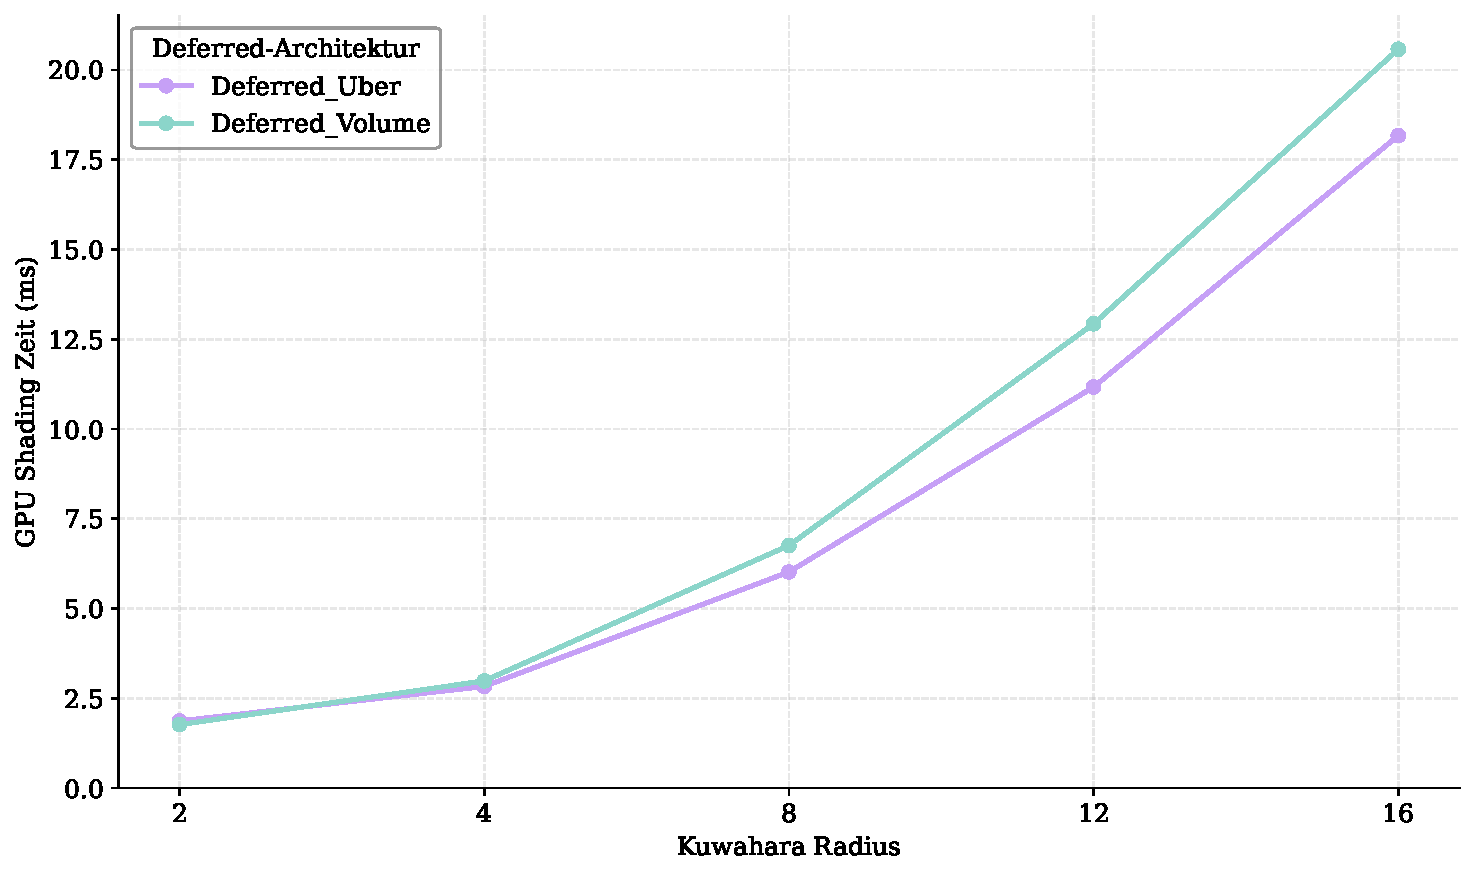
\includegraphics[width=0.85\linewidth]{abbildungen/5_5_3_kernel_bandwidth_scalability}
    \caption[Messung der GPU-Shading-Zeit bei Kuwahara-Radius-Skalierung]{Messung der GPU-Shading-Zeit in Abhängigkeit vom
    Kuwahara-Kernel-Radius (2 bis 16).}
    \label{fig:5_5_3_kernel_bandwidth_scalability}
\end{figure}

% Deduktion.
Die Tatsache, dass die Deferred-Volume-Pipeline im Vergleich zur Deferred-Uber-Pipeline eine
geringere Effizienz aufweist, lässt sich auf eine algorithmische Asymmetrie in der Filter-Implementierung zurückführen.
Wie bereits in Kapitel~\ref{subsec:040202_deferred_uber_pipeline} dargelegt, erfordern die beiden Architekturen
unterschiedliche Ansätze bei der Evaluierung des Kuwahara-Filters.
Die Deferred-Uber-Pipeline operiert mittels \textit{Pre-Lit}-Kuwahara-Filter, um einen algorithmischen Ineffizienz-Kollaps durch
redundante Beleuchtungsberechnungen pro Nachbarpixel zu verhindern.
Sie liest innerhalb der $\mathcal{O}(R^2)$-Schleife ausschließlich Basis-Materialdaten (Albedo und Style-IDs) aus und
berechnet die aufwendige Beleuchtung erst nach Abschluss des Filters für das finale, gemittelte Fragment.
Die Deferred-Volume-Architektur appliziert den Filter im \textit{Resolve}-Pass hingegen auf das bereits
akkumulierte Licht der Szene (\textit{Post-Lit}).
Dies ermöglicht zwar eine \textquote{echtere} Darstellung des Kuwahara-Effektes, erzwingt jedoch innerhalb der innersten
Kuwahara-Schleife zusätzliche Texturlesezugriffe auf den \textit{Light Accumulation Buffer}
(vergleiche Kapitel~\ref{subsec:040203_deferred_volume_pipeline}).

Über die Auswirkungen der asymmetrischen Implementationen des Filters hinaus kann kein signifikanter
Unterschied in der Handhabung von Kernel-Effekten zwischen den untersuchten Deferred-Pipelines festgestellt werden.


\section{{Makro-Benchmark-Synthese}}
\label{sec:0506_macro_eval}

% Kapiteleinleitung.
In der finalen Testreihe erfolgt die Integration aller übergeordneter Einflüsse aus den vorangegangenen Benchmarks in
ein umfassendes praxisnahes Szenario, um die Interaktion der bislang untersuchten Effekte in ihrer Gesamtheit zu
analysieren.
Die nachfolgenden Evaluationen werden in einem Schritt zusammengefasst, bestehen allerdings aus drei verschiedenen
Einzelpässen, in welchen die verschiedenen Einflüsse von Geometrie, Beleuchtung und selektiver Silisierung gemeinsam
betrachtet werden.

% Versuchseinleitung.
Die Makro-Benchmark-Synthese nutzt einen deterministischen Kamera-Flythrough, um die Leistungsfähigkeit der
Architekturen in einem praxisnahen Produktionsszenario zu evaluieren
(vgl.\ Kap~\ref{sec:0404_telemetry_and_benchmark_orchestrator}).
Das zugrunde liegende Szenario generiert eine dichte, prozedurale Umgebung mit 15.000 verteilten Instanzen bei einem
konstanten Detailgrad ($\ac{LOD} = 1$) und vollflächiger Bodenabdeckung.
Dabei ist die räumliche Entropie der Rendering-Stile bewusst auf eine gestreute Verteilung konfiguriert.
Der programmierte Kamera-Flug erstreckt sich über $3.000$ Frames und durchquert die Szenerie auf einem festgelegten Pfad.
Dabei werden kontinuierlich wechselnde Sichtfeldkomplexitäten, stark schwankende Frustum-Culling-Raten sowie variable
Tiefen- und Lichtüberlappungen erzwungen, um eine ganzheitliche und dynamische Belastung der Pipelines zu gewährleisten.
Die Evaluation erfolgt in drei isolierten, aufeinander aufbauenden Pässen zur exakten Dekonstruktion der Leistungskosten.
Die Ergebnisse werden kombiniert dargestellt.
In Pass 1 (\textit{Geometry Baseline}) wird vollständig auf Beleuchtung und Stilisierung verzichtet, um die reine
Grundlast der Geometrieverarbeitung und \ac{G-Buffer}-Initialisierung zu erfassen.
In Pass 2 (\textit{Shading Tax}) werden 250 dynamische Punktlichter als Umgebungsbeleuchtung hinzugefügt, um
die Effizienz der additiven Lichtakkumulation zu messen.
In Pass 3 (\textit{\ac{NPR}-Parity}) werden zusätzlich die hybriden Stilisierungen (Toon-Shading, Gooch-Shading und
Outlines; vgl.\ Kap.~\ref{sec:0403_npr_payloads}) aktiviert, um die kombinierte Auswirkung von Beleuchtungs- und
Entropie-Last zu evaluieren.
Als zentrale Metrik wird in allen Messungen die akkumulierte \ac{GPU}-Gesamtlaufzeit ($t_{\text{GPU}}$) herangezogen.

% Aufbau.
\begin{center}
    \small
    \colorbox{gray!5}{\parbox{0.95\textwidth}{
        \centering
        \vspace{3mm}
        {\sffamily\bfseries\large Versuchs-Setup} \\[2ex]

        \begin{tabularx}{0.9\textwidth}{>{\sffamily}l X}
            Versuchs-Typ:       & Dynamischer Kamera-Flythrough ($3.000$ Frames Gesamtdauer) \\
            Kontrollvariablen:  & $N_{\text{Inst}} = 15.000$, $r_{\text{Spawn}} = 150{,}0$, $LOD = 1$,
            Boden aktiviert, Gestreute Stile ($E_{\text{Spatial}} = \text{Gestreut}$) \\
            \midrule
            \addlinespace
            \quad Pass 1 (Geometry Baseline): & $N_{\text{Light}} = 0$, Alle \ac{NPR}-Effekte deaktiviert \\
            \quad Pass 2 (Shading Tax):       & $N_{\text{Light}} = 250$, Alle \ac{NPR}-Effekte deaktiviert \\
            \quad Pass 3 (\ac{NPR}-Parity):   & $N_{\text{Light}} = 250$, Gooch, Toon und Outlines aktiviert \\

            \addlinespace
            \midrule
            \addlinespace

            Zielgröße:          & \ac{GPU}-Gesamtlaufzeit ($t_{\text{GPU}}$)
        \end{tabularx}
        \vspace{1mm}
    }}
\end{center}

% Beschreibungen.
Die Betrachtung der akkumulierten Einzelpässe in Abbildung~\ref{fig:5_6_cumulative_rendering_cost_combined} schlüsselt
die architektonischen Kostenstrukturen der Rendering-Pipelines detailliert auf.
Im ersten Pass (Geometry Baseline) erweist sich die Forward-Architektur mit einer initialen Ausführungszeit von
\qty{0,51}{\milli\second} als minimal effizienter als die Deferred-Architekturen.
Die Deferred-Pipelines weisen mit \qty{0,68}{\milli\second} (Deferred-Uber) respektive \qty{0,77}{\milli\second}
(Deferred-Volume) die erwartete architektonische Grundlast auf, die durch die initialen Schreibvorgänge in
den \ac{G-Buffer} bedingt ist (vgl.\ Basislast in~\ref{subsec:050302_bandwidth_eval}).
Unter der additiven Zuschaltung von 250 Lichtquellen im zweiten Pass (Shading Tax) kollabiert die Forward-Pipeline unter
der multiplikativen Instruktionslast der Lichtberechnungen und verzeichnet eine massive Zusatzlast von
$+\qty{1,69}{\milli\second}$.
Die Deferred-Pipelines profitieren hier signifikant von der zweidimensionalen Screen-Space-Beleuchtung und fangen die
Rechenlast mit \qty{0,72}{\milli\second} (Deferred-Uber) sowie $+\qty{1,01}{\milli\second}$ (Deferred-Volume)
deutlich effizienter ab (vgl.\ Ergebnisse aus~\ref{subsec:050401_light_count_eval}).
Die Aktivierung der gestreuten \ac{NPR}-Stile im dritten Pass (\ac{NPR}-Parity) offenbart schließlich die
architektonischen Schwächen des Deferred-Uber-Shaders, der durch \textit{Warp Divergence} und Registerdruck
eine Zusatzlast von \qty{0,10}{\milli\second} erfährt (vgl.~\ref{subsec:050501_entropy_eval}).
Das Deferred-Volume-Rendering erweist sich mit einer minimalen Steigerung von lediglich $+\qty{0,03}{\milli\second}$ als
nahezu immun gegen diese stilistische Entropie, während die Forward-Pipeline um weitere $+\qty{0,17}{\milli\second}$
degradiert.
Der zeitliche Verlauf des Kamera-Flythroughs in Abbildung~\ref{fig:5_6_flythrough_variance} bestätigt diese
Beobachtungen über einen Zeitraum von $3.000$ Frames.
Es lässt sich deutlich erkennen, dass die Leistungskurven mit zunehmender Komplexität des Sichtfelds ansteigen.
Sobald die Kamera in die Objekt- und Licht-Wolke eintaucht, können die jeweiligen Spitzen beobachtet werden.

% Ergebnis Graph 1.
\begin{figure}[htbp]
    \centering
    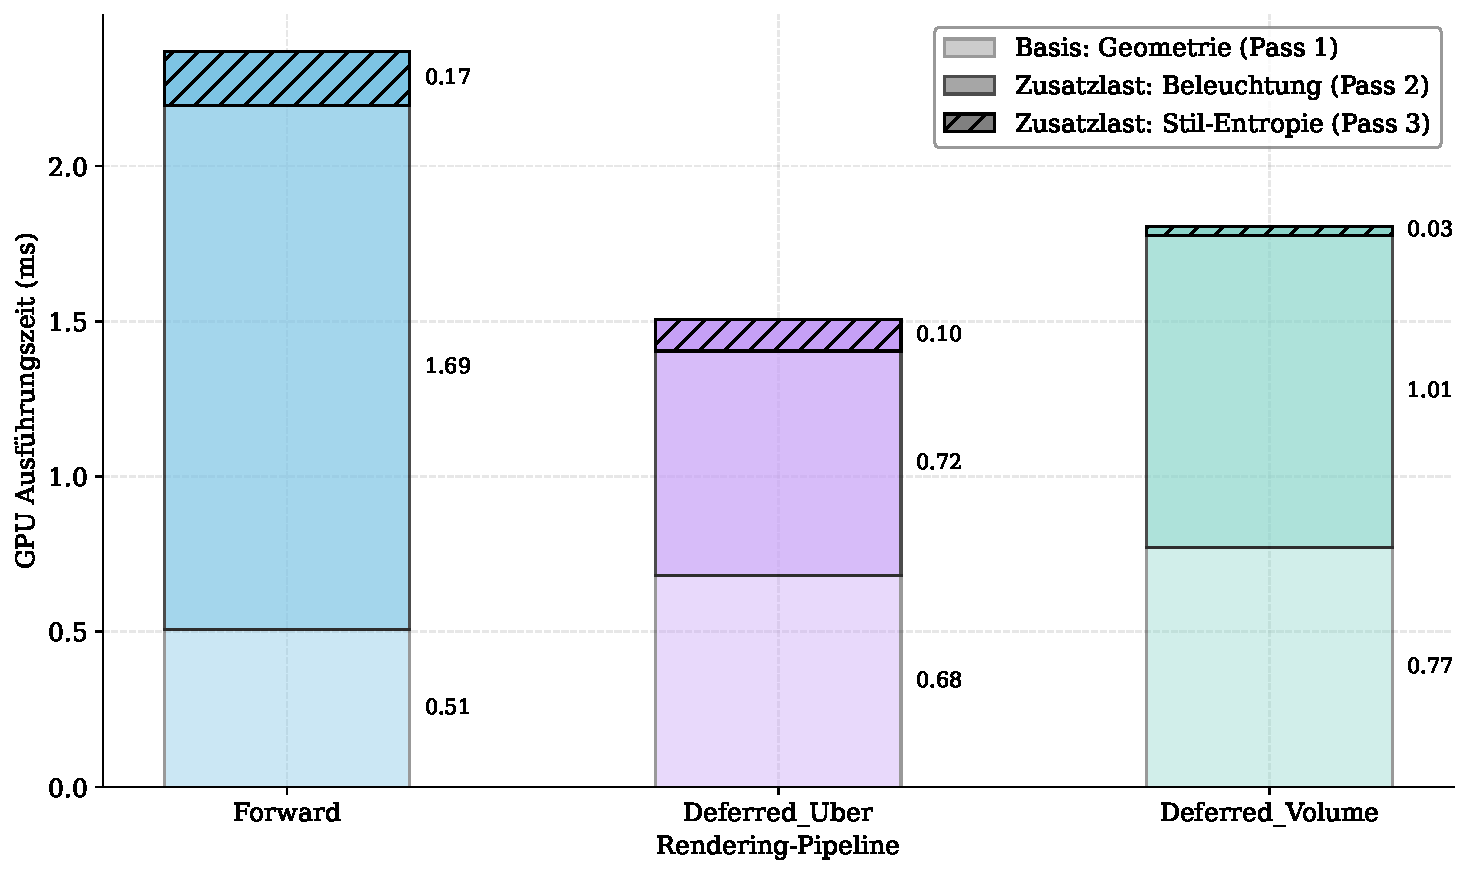
\includegraphics[width=0.85\linewidth]{abbildungen/5_6_cumulative_rendering_cost_combined}
    \caption[Akkumulierte GPU-Ausführungszeit im Makro-Benchmark]{Aufschlüsselung der GPU-Ausführungszeit nach
    Pipeline-Komponenten (Geometrie, Beleuchtung und Stil-Entropie).}
    \label{fig:5_6_cumulative_rendering_cost_combined}
\end{figure}

% Ergebnis Graph 2.
\begin{figure}[htbp]
    \centering
    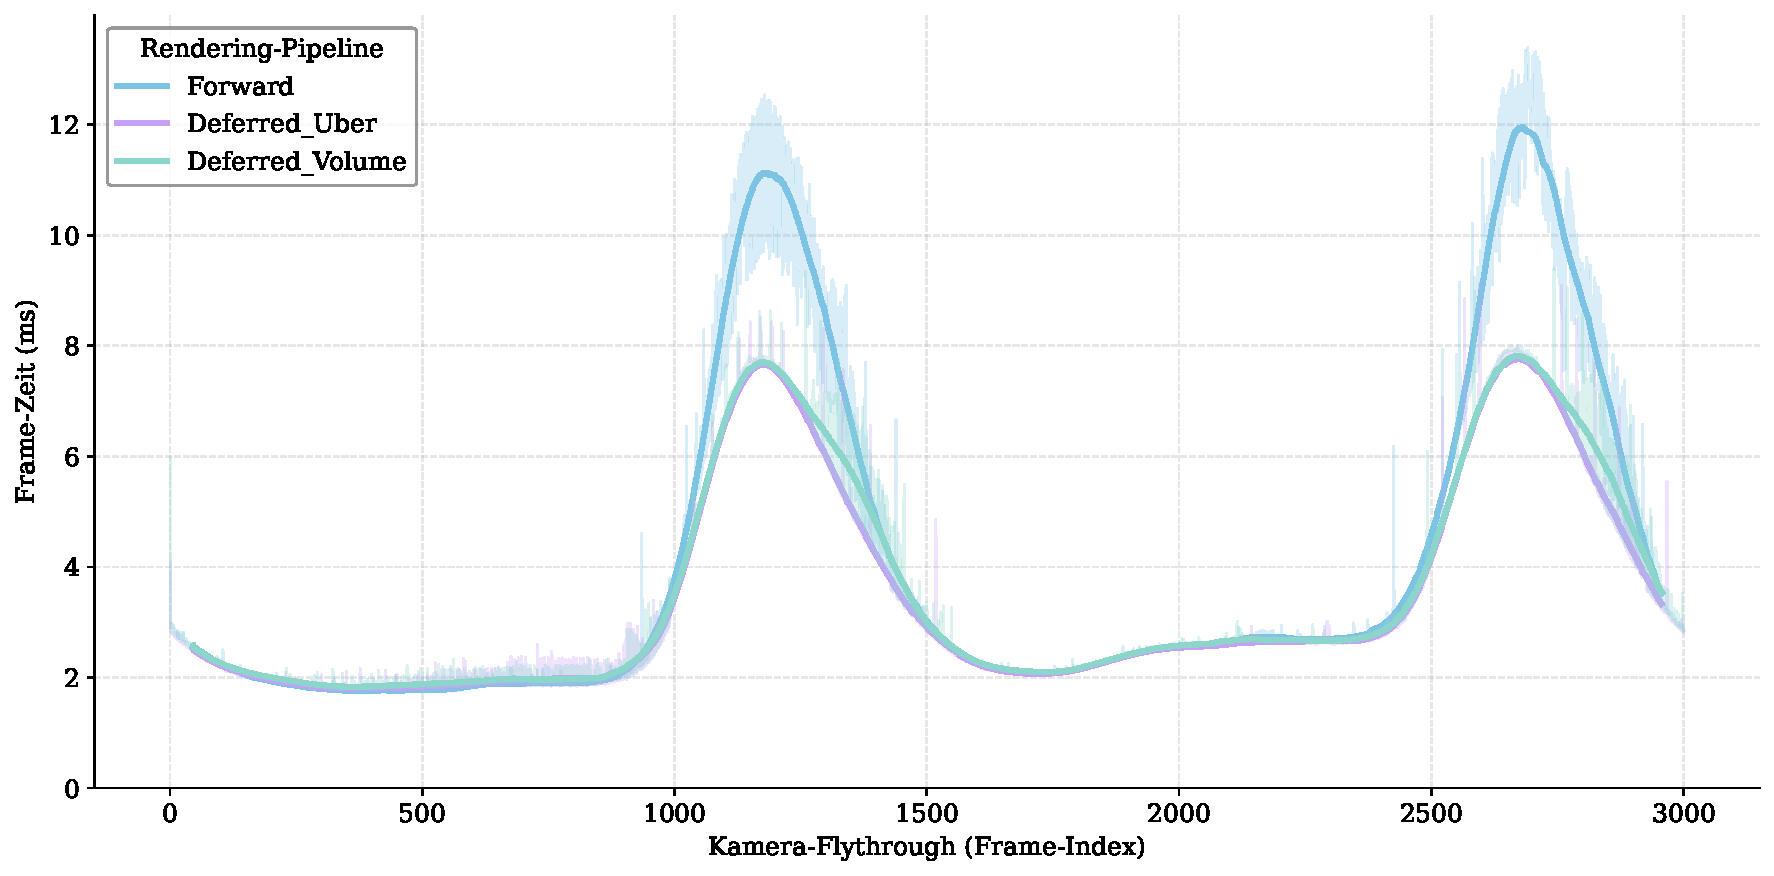
\includegraphics[width=0.85\linewidth]{abbildungen/5_6_flythrough_variance_npr}
    \caption[Frame-Zeit-Verlauf des Kamera-Flythroughs in Makro-Benchmark]{Verlauf der Frame-Zeit über die Dauer von 3000 Frames des
    Kamera-Flythroughs unter kombinierter Geometrie-, Beleuchtungs- und Stil-Last.}
    \label{fig:5_6_flythrough_variance}
\end{figure}

% Vorab-Fazit.
Die Ergebnisse dieser Makro-Synthese vereinen die in den vorangegangenen Evaluierungskapiteln isoliert gewonnenen
Erkenntnisse in einem kohärenten Gesamtbild.
Als primäres Vorab-Fazit lässt sich konstatieren, dass es im Kontext der untersuchten Paradigmen keine universell
überlegene Pipeline-Architektur gibt.
Die Leistungsfähigkeit der einzelnen Architekturen unterliegt einer dynamischen Veränderung, die in direkter
Abhängigkeit zur dominanten Szenenlast steht.
Die naive Forward-Pipeline zeigt eine hohe Effizienz bei der reinen Geometrieverarbeitung und einer geringen Lichtdichte
(vgl.\ Ergebnisse aus~\ref{sec:0502_geometry_eval}).
Aufgrund der untrennbaren Verknüpfung von Geometrieauswertung und Beleuchtungsberechnung kollabiert sie jedoch unter der
multiplikativen Instruktionslast, sobald lichtstarke Produktionsszenarien mit hunderten Lichtquellen gefordert werden
(vgl.\ Ergebnisse aus~\ref{subsec:050401_light_count_eval}).
Die einfache Deferred-Uber-Architektur löst dieses Beleuchtungsproblem effizient im Screen-Space,
scheitert jedoch architektonisch an der \textit{Warp Divergence}, sobald eine hohe stilistische Entropie durch
divergierende \ac{NPR}-Code-Zweige erzwungen wird (vgl.\ Ergebnisse aus~\ref{subsec:050501_entropy_eval}).
Die Deferred-Volume-Architektur umgeht diese Branching-Problematik zwar durch die strikte architektonische
Isolierung der Code-Pfade und Verwendung von Proxy-Geometrien für die Punktlichtquellen, weist jedoch fundamentale
Schwächen in der Speicherbandbreite auf.
Ihr primärer architektonischer Engpass manifestiert sich auf dem \ac{VRAM}-Speicherbus, der durch zahlreiche
additive \ac{RMW}-Zyklen bei extremer räumlicher Überlappung der Lichtquellen gesättigt wird
(vgl.\ Ergebnisse aus~\ref{subsec:050402_light_intensity_and_overlap_eval}).
